\documentclass[fleqn,reqno,10pt]{article}


%========================================
% Packages
%========================================

\usepackage[]{../helpers/mypackages}
%\usepackage[natbib=true,style=authoryear-comp,backend=bibtex,doi=false,url=false]{biblatex}
%\bibliography{MyRefGlobal}
\bibliography{../helpers/MyRefGlobal}
\bibliography{paper} 
\usepackage{../helpers/myenvironments}
\usepackage{../helpers/mycommands}
\usepackage{todonotes}
\usepackage{subcaption}



%========================================
% Standard Layout
%========================================

% Itemize
\renewcommand{\labelitemi}{\large{$\mathbf{\cdot}$}}    % itemize symbols
\renewcommand{\labelitemii}{\large{$\mathbf{\cdot}$}}
\renewcommand{\labelitemiii}{\large{$\mathbf{\cdot}$}}
\renewcommand{\labelitemiv}{\large{$\mathbf{\cdot}$}}
% Description
\renewcommand{\descriptionlabel}[1]{\hspace\labelsep\textsc{#1}}

% Figure Captions
\usepackage{caption} % use corresponding myfiguresize!
\setlength{\captionmargin}{20pt}
\renewcommand{\captionfont}{\small}
\setlength{\belowcaptionskip}{7pt} % standard is 0pt

%========================================
% Additional layout & commands
%========================================


\renewcommand{\Smixed}{\ensuremath{\mathrm{\mathbf{s}}}}
\renewcommand{\Rmixed}{\ensuremath{\mathrm{\mathbf{r}}}}

% Annotations
\newcommand{\mytodo}[2]{\todo[inline,color=yellow,author=#1]{#2}}
\newcommand{\question}[2]{\todo[inline,color=blue,author=#1]{#2}}
\newcommand{\answer}[2]{\todo[inline,color=green,author=#1]{#2}}

\newcommand{\rd}{\acro{rd}} % replicator dynamic
\newcommand{\rmd}{\acro{rmd}} % replicator mutator dynamic
\newcommand{\rdd}{\acro{rdd}} % replicator diffusion dynamic
\newcommand{\RD}{\ensuremath{\mathrm{RD}}} % replicator dynamic
\newcommand{\RDD}{\ensuremath{\mathrm{RDD}}} % replicator diffusion dynamic
\newcommand{\RMD}{\ensuremath{\mathrm{RMD}}} % replicator mutator
                                
\newcommand{\Diff}{\ensuremath{\mathrm{D}}} % Difusion 
\newcommand{\Mutate}{\ensuremath{\mathrm{M}}} % Mutation 

\newcommand{\impairment}{\ensuremath{\alpha}} % impairment
\newcommand{\toler}{\ensuremath{\beta}} % tolerance
\newcommand{\ns}{\ensuremath{n_s}} % number of states

\newcommand{\similarity}{\ensuremath{\mathrm{Sim}}} % similarity function


\title{Vagueness, Noise, and Signaling}
% \author{Michael Franke \and Jos\'e Pedro Correia}
\date{}

\begin{document}

\maketitle

\begin{abstract}
  Signaling games have attracted a lot of attention as models for
  studying the evolution of meaning. One important aspect that is
  nevertheless typically missing from most models in the literature is
  the possibility for vagueness as a feature of successful signaling.
  Complementing recent models that have been proposed to explicitly
  address this limitation, we introduce the replicator diffusion
  dynamic. Provably a special case of the replicator mutator dynamic,
  it implements a versatile and natural integration of, on the one hand, stochastic
  noise in the form of probabilistic confusion of similar stimuli and, on
  the other, evolutionary pressure on optimal signal use.
  Applying the replicator diffusion dynamic to a
  generalization of David Lewis' signaling games, so-called
  similarity-maximizing games, we show that stochastic noise can not
  only lead to vague, yet communicative efficient signal use, but can
  also unify evolutionary outcomes and help avoid suboptimal
  categorization.
\end{abstract}

\section{Introduction}

Many of our concepts and words are vague. A vague category knows clear
cases that fall under it, clear cases that do not, and also so-called
borderline cases. Borderline cases neither clearly apply, nor clearly
not apply, and there may be differences between borderline cases in
terms of how well they represent the category in question. Vagueness
does not seem to dramatically affect the success of everyday
communication, but it is troublesome for some of our theories of
language. This is especially the case for the logico-semantic
tradition of Frege, Russell and the young Wittgenstein which is
challenged by the paradoxes vagueness gives rise to. As can be
expected, many proponents of this tradition have tried to address the
problem, ranging from suggesting that there is nothing wrong with the
classical approach since the problem is of a different nature, as in
Williamson's epistemic view~\citep*{Williamson1994:Vagueness}, to
proposing various kinds of modifications to either semantics, logic,
or both, as in for example supervaluationism
\citep[e.g.][]{Mehlberg1958,Fine1975}, many-valued logic
\citep[e.g.][]{Zadeh1975,Machina1976,Edgington1997}, or paraconsistent
logic \citep[e.g.][]{CobrerosEgre2012:Tolerant-Classi}.

Yet there are other intriguing aspects about vagueness. The
puzzle that we are concerned with here is how vagueness could arise
and be maintained in the first place. This may not seem a particularly
deep issue at first glance, but on closer inspection it is a serious
worry to functionalist accounts that maintain that our concepts and
language use evolved in order to be efficient. Since the existence of
unclear borderline cases seems to entail inefficiency of
categorization or communication, the challenge, succinctly put forward
by \citet{Lipman2009:Why-is-Language}, is to explain how vagueness can
exist despite its obvious and demonstrable functional deficiency under
evolutionary pressure to be optimally expressive.

This problem, call it Lipman's problem, has a conceptual and a
technical side to it. Conceptually, it asks for reasons and general
mechanisms by which we could plausibly conceive of vagueness as
resisting the pressure of evolutionary selection for precision. Such
reasons and general mechanisms are, arguably, not hard to imagine.
But each putative explanation, no matter how plausible intuitively,
must also be checked for internal consistency and its potential to
account for the fact that we see vagueness as a part of a by-and-large
efficient system of categorization and communication. In other words,
not all first-shot rebuttals of Lipman's problem will do. Denying that
there is any functional pressure on efficient communication, for
instance, is a non-starter, because it leaves the relative efficiency
of our communication with vague words entirely unexplained. In sum,
the technical answer to Lipman's problem is to give, ideally, a
conceptually sound model of evolution of categorization or language
use that yields by-and-large efficient categories \emph{and}
vagueness.

A number of authors have recently tried to explain why vagueness
evolved, based on considerations why a vague language might be useful
\citep[e.g.][]{Jaegherde-Jaegher2003:A-Game-Theoreti,Deemter2009:Utility-and-Lan,Jaegherde-JaegherRooijvan-Rooij2010:Strategic-Vague,BlumeBoard2013:Intentional-Vag}. In
contrast to these, others have argued that vagueness is a natural
byproduct of limitations in information processing
\citep[e.g.][]{FrankeJager2010:Vagueness-Signa,OConnor2013:The-Evolution-o,QingFranke2014:Gradable-Adject}. This
paper makes a contribution to the latter line of thought.  Concretely,
we introduce the replicator diffusion dynamics ---a novel variant of
the replicator mutator dynamic--- that integrates stochastic noise on
the differential confusability of similar stimuli. Our main
contribution, therefore, is a technical answer to Lipman's problem in
the sense introduced above. The dynamic proposed here generalizes and
complements previous like-minded accounts. We show that stochastic
noise can not only lead to vague, yet communicative efficient signal
use, but can also unify evolutionary outcomes and help avoid
suboptimal categorization.

The next section introduces the background against which the work
presented here can be appreciated. Section~\ref{sec:repl-diff-dynam}
introduces the replicator diffusion dynamic and elaborates on its
relation with the replicator mutator
dynamic. Section~\ref{sec:exploring-rdd} explores the replicator
diffusion dynamic on the relevant class of generalized signaling games
introduced in
Section~\ref{sec:background}. Section~\ref{sec:discussion} reflects on
the results and compares what has been achieved to related accounts in
more detail. 

\section{Background}
\label{sec:background}

The view that vagueness is a natural concomitant of cognitive
limitations of language users has been formalized in a number of ways,
using evolutionary game theory and certain generalizations of
signaling games, so called \emph{similarity-maximizing games}, or
\emph{sim-max games}, for short
\citep{FrankeJager2010:Vagueness-Signa,OConnor2013:Evolving-Percep,OConnor2013:The-Evolution-o}. Our
contribution is best seen in relation to these accounts, as it also
relies on sim-max games. Let's introduce these first, and then zoom in
on the problem of vagueness.

\subsection{Sim-max games \& conceptual spaces}

Signaling games, as introduced by \citet{Lewis_1969:Convention}, have
a sender and a receiver. The sender knows the true state of the world,
but the receiver does not. The sender can select a signal, or message,
to reveal to the receiver, who then chooses an act. In Lewis' games,
states are maximally distinct from each other and the receiver's acts
are related to them one-to-one. If the receiver chooses the act that
corresponds to the actual state, the play is a success, otherwise a
failure. Certain regular combinations of sender signaling and receiver
reaction make messages meaningful, in the sense that their use is
correlated systematically to certain states or acts. To investigate
the conditions under which such meaning-generating behavior can evolve
is a highly interesting topic that we are only beginning to fully
understand
\citep[e.g.][]{Warneryd1993:Cheap-Talk-Coor,BlumeKim1993:Evolutionary-St,Zollman2005:Talking-to-Neig,Huttegger2007:Evolution-and-t,Pawlowitsch2008:Why-Evolution-d,Barrett2009:The-Evolution-o,Wagner2009:Communication-a,HutteggerSkyrms2010:Evolutionary-Dy,Skyrms2010:Signals,HutteggerZollman2011:Signaling-Games}.

Similarity-maximizing games are generalizations of Lewis' games in
that they allow different states to be more or less similar to one
another, and, roughly put, make success of communication a function of
that similarity. Intuitively speaking, while Lewis' games treated
communicative success as a matter of black and white, sim-max games
allow for a gradient notion of communicative success: the more similar
the receiver's interpretation is to the actual state, the more
successful the play is taken to be. Signaling games with
utility-relevant similarities in the state space are fairly standard
in economics
\citep[e.g.][]{Spence1973:Job-market-sign,CrawfordSobel1982:Strategic-Infor},
but have received particular attention in a more philosophical and
linguistic context for reasons that will become clear presently
\citep{Jager2007:The-Evolution-o,JagerRooijvan-Rooij2007:Language-Struct,JagerMetzger2011:Voronoi-Languag}.

A sim-max game, in the relevant sense here, consists of a set of
states $\States$, a set of messages $\Messgs$ with much fever messages
than states, a prior probability distribution $\Pr \in
\Delta(\States)$ that gives the occurrence probabilities of states, a
similarity metric on states $\similarity \mycolon \States \times
\States \rightarrow \mathds{R}$, and a utility function $\Utils
\mycolon \States \times \States \rightarrow \mathds{R}$. We identify
the receiver's acts with the states of the world, so that the game is
one of guessing the actual state, so to speak. We also assume that
sender's and receiver's interests are alike, so we only have one
utility function. We do not consider message costs, so utilities only
depend on the actual state, and the receiver's response. The
similarity function should satisfy the usual requirements for a
metric:
\begin{align*}
  & \similarity(\mystate{1}, \mystate{2}) \ge 0 &&
  \similarity(\mystate{1}, \mystate{2}) = 0 \Leftrightarrow
  \mystate{1} = \mystate{2} \\
  & \similarity(\mystate{1}, \mystate{2}) = \similarity(\mystate{2},
  \mystate{1}) && \similarity(\mystate{1}, \mystate{2}) \le
  \similarity(\mystate{1}, \mystate{3}) + \similarity(\mystate{3}, \mystate{2})\,.
\end{align*}
The utility function should be a monotonically decreasing function of
similarity:
\begin{align*}
  \similarity(\mystate{1},\mystate{2}) \ge
  \similarity(\mystate{1},\mystate{3}) \ \ \Rightarrow \ \ 
  \Utils(\mystate{1},\mystate{2}) \ge
  \Utils(\mystate{1},\mystate{3})\,.
\end{align*}
To keep matters simple, we here only look at cases where $\States$
contains finitely many points from the unit interval, all of which
have equal probability, and with similarity given by the Euclidean
distance in this one-dimensional space.

\citet{JagerMetzger2011:Voronoi-Languag} showed that the
evolutionarily stable states of sim-max games are remarkably
systematic. Their results were obtained for games with infinitely many
states in $n$-dimensional Euclidean space $\States \subseteq
\mathds{R}^n$ and a quadratic loss function for utilities
$\Utils(\mystate{1}, \mystate{2}) = - (\mystate{1} -
\mystate{2})^2$. For these games, the evolutionarily stable states are
demonstrably so-called Voronoi-languages. Intuitively speaking, a
Voronoi language is a pair of sender and receiver strategies, such
that the sender strategy (quasi-)partitions the state space into
convex categories, while the receiver's interpretations are the
central spots in each category. Figure~\ref{fig:VoronoiLanguage} gives
an example of such a Voronoi-language for a sim-max game with $\States
= [0,1]$, two messages, and a flat prior distribution over states. The
sender uses one message exclusively for all points in the lower half
of the interval and another for all points in the upper half. The
receiver's interpretations of messages are the central points in the
respective intervals.

\begin{figure}
  \centering

  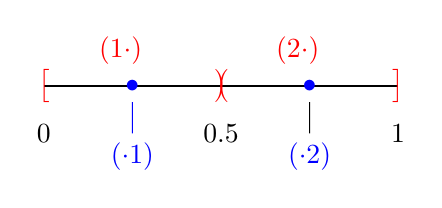
\begin{tikzpicture}[scale=3]

        \begin{scope}

          \draw[-,thick] (0,0) -- (1.5,0);

          \draw (0,0) node {\color{red}{\big{[}}};

          \draw (.75,0) node {\color{red}{\big{)}}};

          \draw (.76,0) node {\color{red}{\big{(}}};

          \draw (1.5,0) node {\color{red}{\big{]}}};

            \draw (.325,.15) node
            {\color{red}{$\Spure(\mymessg{1}  \probbar \cdot)$}};

            \draw (1.075,.15) node
            {\color{red}{$\Spure(\mymessg{2} \probbar \cdot)$}};

            \node at (.375,0) (node1) {\color{blue}{$\bullet$}};

            \node at (.375,-.3) (label1)
            {\color{blue}{${\Rpure}(\cdot \probbar \mymessg{1})$}};

            \draw[-,color=blue] (node1) -- (label1);

            \node at (1.125,0) (node2) {\color{blue}{$\bullet$}};

            \node at (1.125,-.3) (label2)
            {\color{blue}{${\Rpure}(\cdot \probbar \mymessg{2})$}};

            \draw[-] (node2) -- (label2);

            \draw (0,-.2) node {$0$};

            \draw (.75,-.2) node {$0.5$};

            \draw (1.5,-.2) node {$1$};

          \end{scope}
 
        \end{tikzpicture}

        \caption{Example of a Voronoi-language on $\States =
          [0,1]$. The (pure) sender strategy $\Spure \in
          \Messgs^\States$ uses one signal for the lower half, and
          another for the upper half of the unit interval. The (pure)
          receiver strategy $\Rpure \in \States^\Messgs$ selects the
          central elements in the respective intervals.}
  \label{fig:VoronoiLanguage}
\end{figure}


This result is interesting, because it demonstrates that signaling can
impose orderly categories on a metric space, without that being the
ulterior purpose of it all. Sender and receiver can be distinct
entities, whose purpose is to communicate effectively about the actual
state. In that case, evolving Voronoi-languages would explain why
linguistic categories are well-behaved and orderly in the way they
appear to be. More abstractly, sender and receiver can also be thought
of as distinct modules in a single system, where the first module must
discretize the information by selecting a small sample of,
suggestively, category labels. These are passed to a second module
that tries to decode the original information. In this case, evolving
Voronoi-languages would explain why conceptual categories are
well-behaved and orderly in the way that they appear to be
\citep[e.g.][for more on this latter
interpretation]{OConnor2013:Evolving-Percep}.

Seen in this light, sim-max games appear to have the potential of
providing a foundation to approaches in cognitive semantics that rely
on the notion of conceptual spaces.
\citet[][70--77]{Gardenfors2000:Conceptual-Spac}, for example, has
prominently argued that natural categories are convex regions in
conceptual space. If the conceptual space has a suitable metric, then
it is possible to think of these convex categories as derived from a
set of prototypes. Fixing a set of prototypes, we consider the
category corresponding to each prototype $p$ as the set of points that
are more similar to $p$ than to any other
\citep[e.g.][]{OkabeBoots2000:Spatial-Tessell}. In this way,
\citet{Gardenfors2000:Conceptual-Spac} argues, an efficient
categorization system can be obtained: storing the prototypes lets us
recover the categories without having to store each category's
extension. However, what is left unexplained so far, is where the
prototypes come from, and why we would not see just any distribution
of prototypes as an equally efficient classification system. This is
where sim-max games can contribute a principled approach to deriving,
in an independent way, not only convex categories but also
prototypical exemplars belonging to them.


\subsection{Vague signaling in sim-max games}

This brief outline of an approach to conceptual categorization using
sim-max games leaves many problems unaddressed. One of them is that
natural categories for continuously variable stimuli, like shades of
color, pitch heights, spatial dimension and the like, do not have
unique, point-valued prototypes and clear category boundaries. We
would like to account for the possibility of such vagueness, and that
means in particular for the following criteria
\citep[e.g.][]{Sainsbury1991:Is-There-Higher,KeefeSmith1997:Vagueness:-A-Re,Smith2008:Vagueness-and-D}:
(i) clear positive examples of a vague category should show a
gradient, perhaps smooth, transition to clear negative examples to
accommodate also higher-order vagueness; (ii) prototypes should
likewise be gradient regions, peaking at the center of the vague
category they represent.


\citet{DouvenDecock2011:Vagueness:-A-Co} show that
\citeauthor{Gardenfors2000:Conceptual-Spac}'s conceptual spaces
approach can be extended to account for the existence of borderline
cases. From the assumption that prototypes are not unitary points, but
extended, yet convex regions in conceptual space,
\citeauthor{DouvenDecock2011:Vagueness:-A-Co} give a construction
algorithm that yields ``collated Voronoi diagrams'' with thick,
extended boundaries representing borderline regions. Building on this
work, \citet{DecockDouven2012:What-is-Graded-} show further how it is
possible to arrive at higher-order vagueness and degrees of category
membership, by, essentially, weighing in the distance of different
borderline cases to various prototypical regions. This accounts for
the first of the two desiderata mentioned above, but still assumes
that crisp non-gradient prototype regions must be pre-given.

An alternative approach is taken by
\citet{FrankeJager2010:Vagueness-Signa} and
\citet{OConnor2013:The-Evolution-o} who show how the above desiderata
can be met by evolving strategies in sim-max games for various types
of solution concepts. These can be divided into micro- and macro-level
approaches. Micro-level approaches look at adaptive behavior of
individual agents. Usually, changes in the behavioral dispositions of
agents occur after every single interaction. In contrast, macro-level
approaches outline more abstract, aggregate dynamics, happening in a
population of agents, or otherwise abstracting from seemingly
irrelevant detail. Usually, a macro-level dynamic captures changes of
frequencies of behavioral types in the population over time.

As for micro-dynamics, \citet{FrankeJager2010:Vagueness-Signa} show
how limited memory of past interactions can lead to vague signal use,
when averaging over a single agent's behavior over time or over the
momentary behavior of a population of several language
users. \citet{OConnor2013:The-Evolution-o} introduces a variant of
reinforcement learning that entails a low-level form of stimulus
generalization. Agents update their behavior after each round of play
in such a way that states similar to the one that actually occurred
are subject to behavioral adjustment as well. (A more detailed
discussion of alternative approaches is deferred until
Section~\ref{sec:discussion}, where we can compare them better with the
system introduced in this paper.)

\citet{FrankeJager2010:Vagueness-Signa} also consider a macro-level
approach, using the notion of a \emph{quantal response}. A quantal
response function is a probabilistic choice rule that formalizes the
idea that agents make small mistakes when calculating the expected
utility of choice options. In aggregation, these probabilistic
mistakes lead to systematic ``trembles'' that produce vague signal
use. The approach we take here is superficially similar, but there are
crucial differences. For one, we adopt a dynamic perspective by
looking at limited-time outcomes of a dynamic process. For another, we
demonstrate in Section~\ref{sec:discussion} that quantal responses can
give rise to counterintuitive predictions. These counterintuitive
examples suggest that vagueness in sim-max games is not convincingly
explained by appeal to mistakes in calculating expected utility, but
rather, as we assume here, as the result of confusing similar
states.




%%% Local Variables: 
%%% mode: latex
%%% TeX-master: "paper"
%%% TeX-PDF-mode: t
%%% End:





\section{Noise-perturbed replicator dynamic}

\subsection{Preliminaries}

\paragraph{Notation.} Fix a signaling game with states $\States$,
messages $\Messgs$ and acts $\Acts$. % Let $\Util_{\sen,\rec} \mycolon
% \States \times \Messgs \times \Acts \rightarrow \mathds{R}$ be the
% player's utility function.

Pure sender (receiver) strategies are functions $\Spure \in
\Messgs^\States$ ($\Rpure \in \Acts^\Messgs$). Mixed sender (receiver)
strategies are functions $\Smixed \in \Delta(\Messgs^\States)$
($\Rmixed \in (\Acts^\Messgs)$). The latter give the relative
population frequencies of the former. We write $\Smixed_i$ for the
frequency $\Smixed(\Spure_i)$ of pure strategy $\Spure_i$ (also for
the receiver).

Let the sender's (receiver's) behavioral strategies be functions in
$\Sstrat \in \Delta(\Messgs)^\States$ ($\Rstrat \in
\Delta(\Acts)^\Messgs$). Every mixed strategy $\Smixed$ converts to a
unique behavioral strategy defined by:
\begin{align*}
  \Sstrat(\messg \probbar \state) = \sum_{\Spure(\state) = \messg} \Smixed(\Spure)\,.
\end{align*} 
Let $G$ be this mapping from mixed to behavioral strategies. Notice
that $G$ is \emph{not} an injection, as many mixed strategies map onto
the same behavioral strategy.

For behavioral strategies, let $\EU(\messg, \state, \Rstrat)$ and
$\EU(\act, \messg, \Sstrat)$ be the players' expected utilities of
each action in each choice point as usual. For mixed strategies we
define the players' fitness in the usual manner. Let $F_i^{\Rmixed}$
be $\Spure_i$'s fitness given $\Rmixed$ and $F_i^{\Smixed}$ be
$\Rpure_i$'s fitness given $\Smixed$. Then $\Phi(\Smixed,\Rmixed) =
\sum_{k} \Smixed_k \cdot F_k^{\Rmixed}$ is the average fitness in the
sender population and $\Phi(\Rmixed,\Smixed) = \sum_{k} \Rmixed_k
\cdot F_k^{\Smixed}$ the average fitness in the receiver population.

\paragraph{Replicator dynamics in pure strategies.} The two-population
(non-payoff adjusted) continuous replicator dynamics in pure
strategies is defined as:
\begin{align*}
  \dot{\Smixed_i} & = \Smixed_i \cdot \left ( F_i^{\Rmixed} -
  \Phi(\Smixed,\Rmixed) \right ) &   \dot{\Rmixed_i} &  = \Rmixed_i \cdot \left ( F_i^{\Smixed} -
  \Phi(\Rmixed,\Smixed) \right ) \,.
\end{align*}
The discrete time version is given by: 
\begin{align*}
  \Smixed_i' & = \frac{\Smixed_i \cdot
  F_i^{\Rmixed}}{ \Phi(\Smixed,\Rmixed)} &     \Rmixed_i' & = \frac{\Rmixed_i \cdot
  F_i^{\Smixed}}{ \Phi(\Rmixed,\Smixed)} \,.
\end{align*}


\paragraph{Replicator-mutator equation.} Let $Q$ be a row-stochastic
mutation matrix where $Q_{ji}$ gives the probability that pure sender
strategy $\Spure_j$ mutates into $\Spure_i$. Similarly, let $R$ be a
row-stochastic mutation matrix where $R_{ji}$ gives the probability
that pure receiver strategy $\Rpure_j$ mutates into $\Rpure_i$.

The two-population (non-payoff adjusted) continuous replicator-mutator
dynamics, is then given by::
\begin{align*}
  \dot{\Smixed_i} & = \sum_{j}  Q_{ji} \cdot \Smixed_j
    \cdot F_j^{\Rmixed} - \Smixed_i \cdot \Phi(\Smixed,\Rmixed) &
    \dot{\Rmixed_i} & = \sum_{j}  R_{ji} \cdot \Rmixed_j
    \cdot F_j^{\Smixed} - \Rmixed_i \cdot \Phi(\Rmixed,\Smixed) \,.
\end{align*}
\begin{claim} A discrete time version of the above replicator mutator
  dynamics is:
  \begin{align*}
    \Smixed_i' & = \sum_{j} Q_{ji} \frac{\Smixed_j \cdot
      F_j^{\Rmixed}}{ \Phi(\Smixed,\Rmixed)} & \Rmixed_i' & = \sum_{j}
    R_{ji} \frac{\Rmixed_j \cdot F_j^{\Smixed}}{
      \Phi(\Rmixed,\Smixed)}\,.
  \end{align*}
\end{claim}

\begin{proof}
  It suffices to check either sender or receiver part. Focusing on the
  former, we need to show that the continuous version is derivable
  from the discrete version if the discrete update steps get
  infinitely small so that:
  \begin{align*}
    \dot{\Smixed_i} & = \Smixed_i' - \Smixed_i = \sum_{j} Q_{ji}
    \frac{\Smixed_j \cdot F_j^{\Rmixed}}{ \Phi(\Smixed,\Rmixed)} -
    \Smixed_i = \sum_{j} \Smixed_j \left ( \frac{ Q_{ji} \cdot
        F_j^{\Rmixed}}{ \Phi(\Smixed,\Rmixed)} - \Smixed_i \right ) \\
    & = \sum_{j} \Smixed_j \left ( \frac{ Q_{ji} \cdot
        F_j^{\Rmixed} - \Smixed_i \cdot \Phi(\Smixed,\Rmixed)}{ \Phi(\Smixed,\Rmixed)}  \right )
  \end{align*}
  As $\Phi(\Smixed,\Rmixed)$ is a constant rate of change, we can drop
  it to derive the non-payoff adjusted continuous version above,
  since:
  \begin{align*}
    & \sum_{j} \Smixed_j \left ( Q_{ji} \cdot
        F_j^{\Rmixed} - \Smixed_i \cdot \Phi(\Smixed,\Rmixed)  \right
      ) =     \sum_{j} \Smixed_j  Q_{ji} \cdot
        F_j^{\Rmixed} - \sum_{j} \Smixed_j \cdot \Smixed_i \cdot
        \Phi(\Smixed,\Rmixed) \\
       = &    \sum_{j} \Smixed_j  Q_{ji} \cdot
        F_j^{\Rmixed} - \Smixed_i \cdot
        \Phi(\Smixed,\Rmixed) 
  \end{align*}
\end{proof}

The discrete time replicator-mutator dynamics has a nice sequential
update property: first we compute the fitness-driven change according
to the standard replicator dynamics; then we compute the perturbation
from mutation.

\subsection{Noise-perturbed replicator dynamics}

We look at signaling games with $\States = \Acts$ and fix a confusion
matrix $C$, which is a row-stochastic matrix whose elements $C_{ij}$
give the probability that $\state_i$ is perceived as
$\state_j$. Define players average utility at each choice point given
the opponent's strategy as:
\begin{align*}
  \Phi(\state,\Rstrat) & = \sum_{\messg} \Sstrat(\messg \probbar \state) \cdot
\EU(\messg,\state,\Rstrat) &
\Phi(\messg,\Sstrat) & = \sum_{\state} \Rstrat(\state \probbar \messg)
\cdot \EU(\state,\messg,\Sstrat)\,.
\end{align*}
The discrete noise-perturbed replicator dynamics on behavioral
strategies proposed by \citet{Correia2013:The-Bivalent-Tr} is:
\begin{align*}
  \Sstrat'(\messg \probbar \state_i) & = \sum_{j} C_{ji} \cdot
  \frac{\Sstrat(\messg \probbar \state_j) \cdot
    \EU(\messg,\state_j,\Rstrat)} {\Phi(\state_j,\Rstrat)} \\
    \Rstrat'(\state_i \probbar \messg) & = \sum_{j} C_{ji} \cdot
  \frac{\Rstrat(\state_j \probbar \messg) \cdot
    \EU(\state_j,\messg,\Sstrat)} {\Phi(\messg,\Sstrat)}  \,.
\end{align*}
Notice that this update is also sequential: first we calculate an
update according to the standard replicator dynamics (in behavioral
strategies), then we compute the perturbation from perceptual noise.


\subsection{Exploring the relation}

We will show that the noise-perturbed replicator dynamics defined
above is the behavioral-strategy analogue to the replicator-mutator
dynamics when the only source of mutation is perceptual confusion of
states. Since, in general, the replicator dynamics in two-populations
is not equivalent in its formulations for behavioral and mixed
strategies \citep{Cressman2003:Evolutionary-Dy}, we abstract from the
dynamics and look only at the effect of mutation and
noise-perturbation. This is justified given the above mentioned
sequential nature of both dynamics.

Let the mutation $Q(\Smixed)$ ($R(\Rmixed)$) of a mixed sender
(receiver) strategy be another mixed sender (receiver) strategy
defined by:
\begin{align*}
  Q(\Smixed)_i & =  \sum_j  \Smixed_j \cdot
  Q_{ji} &   R(\Rmixed)_i & =  \sum_{j}  \Rmixed_j \cdot
  R_{ji} \,.
\end{align*}
We would like to compare this to the noise perturbation $C(\Sstrat)$
($C(\Rstrat)$) of behavioral strategy $\Sstrat$ ($\Rstrat)$, which is
another behavioral strategy given by:
\begin{align*}
  C(\Sstrat)(\messg \probbar \state_i) & = \sum_{j} C_{ji} \cdot
  \Sstrat(\messg \probbar \state_j) & C(\Rstrat)(\state_i \probbar
  \messg) & = \sum_{j} C_{ji} \cdot \Rstrat(\state_j \probbar \messg)
  \,.
\end{align*}

We hypothesize that a confusion matrix $C$ should give rise to a
unique mutation matrix $Q^C$ so that whenever $G(\Smixed) = \Sstrat$
we also have $G(Q^C(\Smixed)) = C(\Sstrat)$. Similarly, for the
receiver.

\paragraph{Confusion-based mutations.} There are natural conversions
of $C$ into $Q^C$ and $R^C$. The case for the receiver is easier, so
we start with that.

The probability that $\Rpure$ mutates into $\Rpure'$ is the product of
the probabilities for each $\messg$ that $\Rpure(\messg)$ is perceived
as $\Rpure'(\messg)$. Abusing notation, by refer to the index of
$\Rpure(\messg)$ and $\Rpure'(\messg)$ with $\Rpure(\messg)$ and
$\Rpure'(\messg)$ directly, we define:
\begin{align*}
  R^C_{ji} = \prod_{\messg} C_{\Rpure(\messg)\Rpure'(\messg)}\,.
\end{align*}

Now look at the sender. If $\Spure_j(\state_k)=\messg$ and
$\Spure_i(\state_k)=\messg'$, then the probability of confusion at
state $\state_k$ is given by the chance that $\state_k$ is perceived
as a state $\state_l$ which $\Spure_j$ would map onto $\messg'$. The
overal probability that $\Spure_j$ mutates into $\Sstrat_i$ is the
product of these chances for all states. So, define:
\begin{align*}
  Q^C_{ji} = \prod_{\state_k} \sum_{\state_l \in
    \Spure_j^{-1}(\Spure_i(\state_k))} C_{kl}\,.
\end{align*}

For example, consider a signaling game with two states and two
messages. Let the confusion matrix be:
\begin{align*}
  C=
  \begin{pmatrix}
    .8 & .2 \\
    .2 & .8 
  \end{pmatrix}\,.
\end{align*}
The resulting mutation matrices are:
\begin{align*}
S^C & = \bordermatrix{ ~ & 11 & 12 & 21 & 22 \cr
                      11 & 1 & 0 & 0 & 0 \cr
                      12 & .16 & .64 & .04 & .16 \cr
                      21 & .16 & .04 & .64 & .16 \cr
                      22 & 0 & 0 & 0 & 1 \cr}
&                    
  R^C & = \bordermatrix{ ~ & 11 & 12 & 21 & 22 \cr
                      11 & .64 & .16 & .16 & .04 \cr
                      12 & .16 & .64 & .04 & .16 \cr
                      21 & .16 & .04 & .64 & .16 \cr
                      22 & .04 & .12 & .12 & .64 \cr}\,.
\end{align*}
Here, a pair like $21$, for example, refers to a pure sender strategy
with $\Spure(\state_1=\messg_2$ and $\Spure(\state_2) =
\messg_1$. Similarly for the receiver.

\medskip

\todo[inline]{necessary to prove that mutation matrices are row-stochastic?}

\todo[inline]{maybe worthwhile to think about general properties of
  the mutation matrices that ensue from perceptual confusion?}

\medskip

\begin{theorem}
  \label{thm:sender-eq}
  If $G(\Smixed) = \Sstrat$, then $G(Q^C(\Smixed)) = C(\Sstrat)$.
\end{theorem}


\begin{theorem}
  \label{thm:receiver-eq}
  If $G(\Rmixed) = \Rstrat$, then $G(R^C(\Rmixed)) = C(\Rstrat)$.
\end{theorem}

%%% Local Variables: 
%%% mode: latex
%%% TeX-master: "paper"
%%% TeX-PDF-mode: t
%%% End:





\section{Simulations}

In order to study the long-term behavior of the noise-perturbed sim-max games, we conducted computer simulations for different combinations of initial parameters.
Namely, we were interested in investigating the impact of different values of impairment and its relation with the size of the state space.
\mytodo{JPC}{Justify why size of state space is interesting}

\subsection{Metrics}
\label{sec:metrics}
To be able to quantitively analyze the results of our simulations, we define a number of metrics to capture different characteristics of sim-max languages.

\paragraph{Entropy.}
This classic information-theoretic metric captures the amount of uncertainty in a signaling strategy.
The most natural way to define it is in terms of mixed strategies rather than behavioral strategies.
Let us recall that mixed sender (receiver) strategies are functions $\Smixed \in \Delta(\Messgs^\States)$ ($\Rmixed \in (\Acts^\Messgs)$).
We can define the entropy of a sender strategy as
\begin{align*}
  E(\Smixed) = \sum_{\Spure \in \Messgs^\States} \Smixed(\Spure) \cdot \log(\Smixed(\Spure))
\end{align*} 
and the entropy of a receiver strategy as
\begin{align*}
  E(\Rmixed) = \sum_{\Rpure \in \Acts^\Messgs} \Rmixed(\Rpure) \cdot \log(\Rmixed(\Rpure)) \,.
\end{align*} 
These metrics are computationally expensive to calculate, since the size of the domain over which the sum is computed grows exponentially with the number of choice points.
Therefore, we converted\footnote{See Appendix~\ref{sec:proofs}.} the above definitions into equivalent metrics defined in terms of behavioral strategies.
These are as follows:
\begin{align*}
  E(\Sstrat) = -\sum_{\state \in \States} \sum_{\messg \in \Messgs} \Sstrat(\messg \probbar \state) \cdot \log(\Sstrat(\messg \probbar \state))
\end{align*} 
\begin{align*}
  E(\Rstrat) = -\sum_{\messg \in \Messgs} \sum_{\act \in \Acts} \Rstrat(\act \probbar \messg) \cdot \log(\Rstrat(\act \probbar \messg)) \,.
\end{align*}
The metrics are lower bounded by $0$ and upper bounded by, respectively, $\log(|\Messgs^\States|) = |\States| \cdot \log(|\Messgs|)$ and $\log(|\Acts^\Messgs|) = |\Messgs| \cdot \log(|\Acts|)$, thus we can normalize them by dividing by these values.

\paragraph{Informativity.}
\mytodo{JPC}{Informativity is perhaps a bad name for the receiver...}
The quantity of information in a signal is an old notion that also goes back to the start of information theory.
Skyrms~\citet[ch.~3]{Skyrms2010:Signals} discusses its use in the context of signaling games.
The main idea is that we can quantify the amount of information about a state $\state$ in a message $\messg$ via the relation between the probability of the state given the message $\Pr(\state \,|\, \messg)$ and the unconditional probability of the state $\Pr(\state)$.
Following Bayes' theorem, we can express $\Pr(\state \,|\, \messg)$ as $\frac{\Pr(\state) \cdot \Pr(\messg \,|\, \state)}{\Pr(\messg)}$.
We then have $\Pr(\messg \,|\, \state) = \Sstrat(\state,\messg)$ and $\Pr(\messg) = \sum_{\state^\prime \in \States} \Pr(\state^\prime) \cdot \Sstrat(\state^\prime,\messg)$.
Finally, we equate sender infomativity with the average overall information about states in each signal.
Based on the definition by Skyrms~\citet[p.~36]{Skyrms2010:Signals}, and the considerations above, we define sender informativity as follows:
\begin{align*}
  I(\Sstrat) = \frac{1}{|\Messgs|} \sum_{\messg \in \Messgs} \sum_{\state \in \States} \frac{\Pr(\state) \cdot \Sstrat(\state,\messg)}{\sum_{\state^\prime \in \States} \Pr(\state^\prime) \cdot \Sstrat(\state^\prime,\messg)} \cdot \log \left(\frac{\Sstrat(\state,\messg)}{\sum_{\state^\prime \in \States} \Pr(\state^\prime) \cdot \Sstrat(\state^\prime,\messg)} \right) \,.
\end{align*}
Conversely, we can quantify the amount of information about an act in a message.
We equate receiver informativity with the average overall information about acts in each signal.
Based on Skyrms' definition~\citet[p.~39]{Skyrms2010:Signals}, we define receiver informativity as follows:
\begin{align*}
  I(\Sstrat,\Rstrat) = \frac{1}{|\Messgs|} \sum_{\messg \in \Messgs} \sum_{\act \in \Acts} \Rstrat(\messg,\act) \cdot \log \left(\frac{\Rstrat(\messg,\act)}{\sum_{\state \in \States} \Pr(\state) \cdot \sum_{\messg^\prime \in \Messgs} \Sstrat(\state,\messg^\prime) \cdot \Rstrat(\messg^\prime,\act)} \right) \,.
\end{align*}
Both metrics are bounded between $0$ and $1$.

\paragraph{Voronoiness.}
This metric aims to quantify how close a strategy is to being a part of a Voronoi tessallation of the state space.
Recalling the results by \cite{Jager2007}, the stable outcomes of a population of agents playing a similarity-maximization game using pure strategies and evolving according to the replicator dynamics are those where ``the sender strategy is consistent with the Voronoi tessallation that is induced by the image of the receiver strategy.''~(\cite{Jager2007}, p. 562).
\mytodo{JPC}{Explain further?}
Given we are working with behavioral strategies, rather than pure strategies, and that we perform numerical simulations, rather than calculate analytical results, instead of looking into a binary criterion of whether a simulation result is such a Voronoi tessallation of the state space or not, we want a more progressive metric to characterize that in terms of degrees.
With that in mind, and given that this metric only makes sense for $\Acts = \States$, we define Voronoiness as follows.
Let $\pi(\Rstrat, \messg) = \argmax_{\state \in \States}\Rstrat(\messg,\state)$ be the prototype of a message $\messg \in \Messgs$, then
\begin{multline*}
  V(\Sstrat, \Rstrat) = \sum_{\state \in \States} \sum_{\messg_1 \in \Messgs} \sum_{\messg_2 \in \Messgs} \textrm{if } s(\state, \pi(\Rstrat, \messg_1)) > s(\state, \pi(\Rstrat, \messg_2)) \bicond \Sstrat(\state, \messg_1) > \Sstrat(\state, \messg_2) \textrm{ then } 1 \textrm{ else } 0
\end{multline*}
is the Voronoiness of the sender strategy $\Sstrat$ given the receiver strategy $\Rstrat$ and
\begin{align*}
  V(\Rstrat) = \sum_{\messg \in \Messgs} \sum_{\state_1 \in \States} \sum_{\state_2 \in \States} \textrm{if } s(\state_1, \pi(\Rstrat, \messg)) > s(\state_2, \pi(\Rstrat, \messg)) \bicond \Rstrat(\messg, \state_1) > \Rstrat(\messg, \state_2) \textrm{ then } 1 \textrm{ else } 0
\end{align*}
is the Voronoiness of the receiver strategy $\Rstrat$.
\mytodo{JPC}{Give some intuitions on these?}
The metrics are lower bounded by $0$ and upper bounded by, respectively, $|\States| \times |\Messgs|^2$ and $|\Messgs| \times |\States|^2$, thus we can normalize them by dividing by these values.

\subsection{Methodology}
\newcommand{\impairment}{\alpha}
In our simulations we focus on a concrete setup in line with \cite{Correia2013:The-Bivalent-Tr}.
Namely, we define a similarity-maximization game with $\States = \Acts$, where $\States$ is a discrete set of equidistant points within the unit interval $[0,1]$, including the boundaries (thus we always use $n \geq 2$).
As similarity metric $s:\States \times \States \rightarrow [0,1]$, we use a negative exponential of the of the square distance, \emph{i.e.}~for $\state,\state^\prime \in \States$:
\begin{align*}
  s(\state,\state^\prime) =
    \begin{cases}
    1 & \textrm{if } \impairment = 0 \textrm{ and } \state = \state^\prime \\
    0 & \textrm{if } \impairment = 0 \textrm{ and } \state \neq \state^\prime \\
    e^{-\frac{\lVert \state - \state^\prime \rVert ^2}{\impairment^2}} & \textrm{otherwise} \\
    \end{cases}
\end{align*}
where $\impairment$ is an \emph{impairment} factor.
Here we deviate from \cite{Correia2013:The-Bivalent-Tr} by working with impairment $\impairment$ rather than acuity $\theta$, since we are interested in exploring the case of having $0$ impairment, and acuity does not have a natural maximum as defined.
Confusion is directly related with similarity, \emph{i.e.}~the more similar two states are, the more likely an agent is to perceive one as the other.
For simplicity, we equate one with the other by defining $C_{ij} = s(\state_i,\state_j)$.

We run the noise-perturbed replicator dynamics with random initial strategies $\Sstrat_0$ and $\Rstrat_0$ until a convergence criterion is met, namely that the total absolute change in both sender and receiver strategies does not amount to more than $0.01$, \emph{i.e.}:
\begin{align*}
  \sum_{\state \in \States} \sum_{\messg \in \Messgs} \left| \Sstrat^\prime(\state,\messg) - \Sstrat(\state,\messg) \right| < 0.01
\end{align*}
and
\begin{align*}
  \sum_{\messg \in \Messgs} \sum_{\state \in \States} \left| \Rstrat^\prime(\messg,\state) - \Rstrat(\messg,\state) \right| < 0.01 \,.
\end{align*}

We perform a parameter sweep with size of the state space $n \in \{10,
50, 90, 130\}$ and impairment $\impairment \in \{0, 0.1, 0.2, 0.3,
0.4, 0.5\}$.
For each parameter combination, we perform $100$ trials and record the values of each of the metrics introduced in Section~\ref{sec:metrics} after convergence, as well as two additional indicators: number of iterations taken until convergence, and the normalized expected utility.
Expected utility is normalized by dividing by the expected utility of the theoretical optimum without impairment, \emph{i.e.}~a Voronoi tessalation of the state space. 

\subsection{Results}
In order to visualize the impact of the impairment factor on the outcome of simulations, we plot in Figure~\ref{fig:metrics-boxplots} the distribution of each of the measurements per impairment value.
%
\begin{figure}
        \centering
        \begin{subfigure}{0.45\textwidth}
                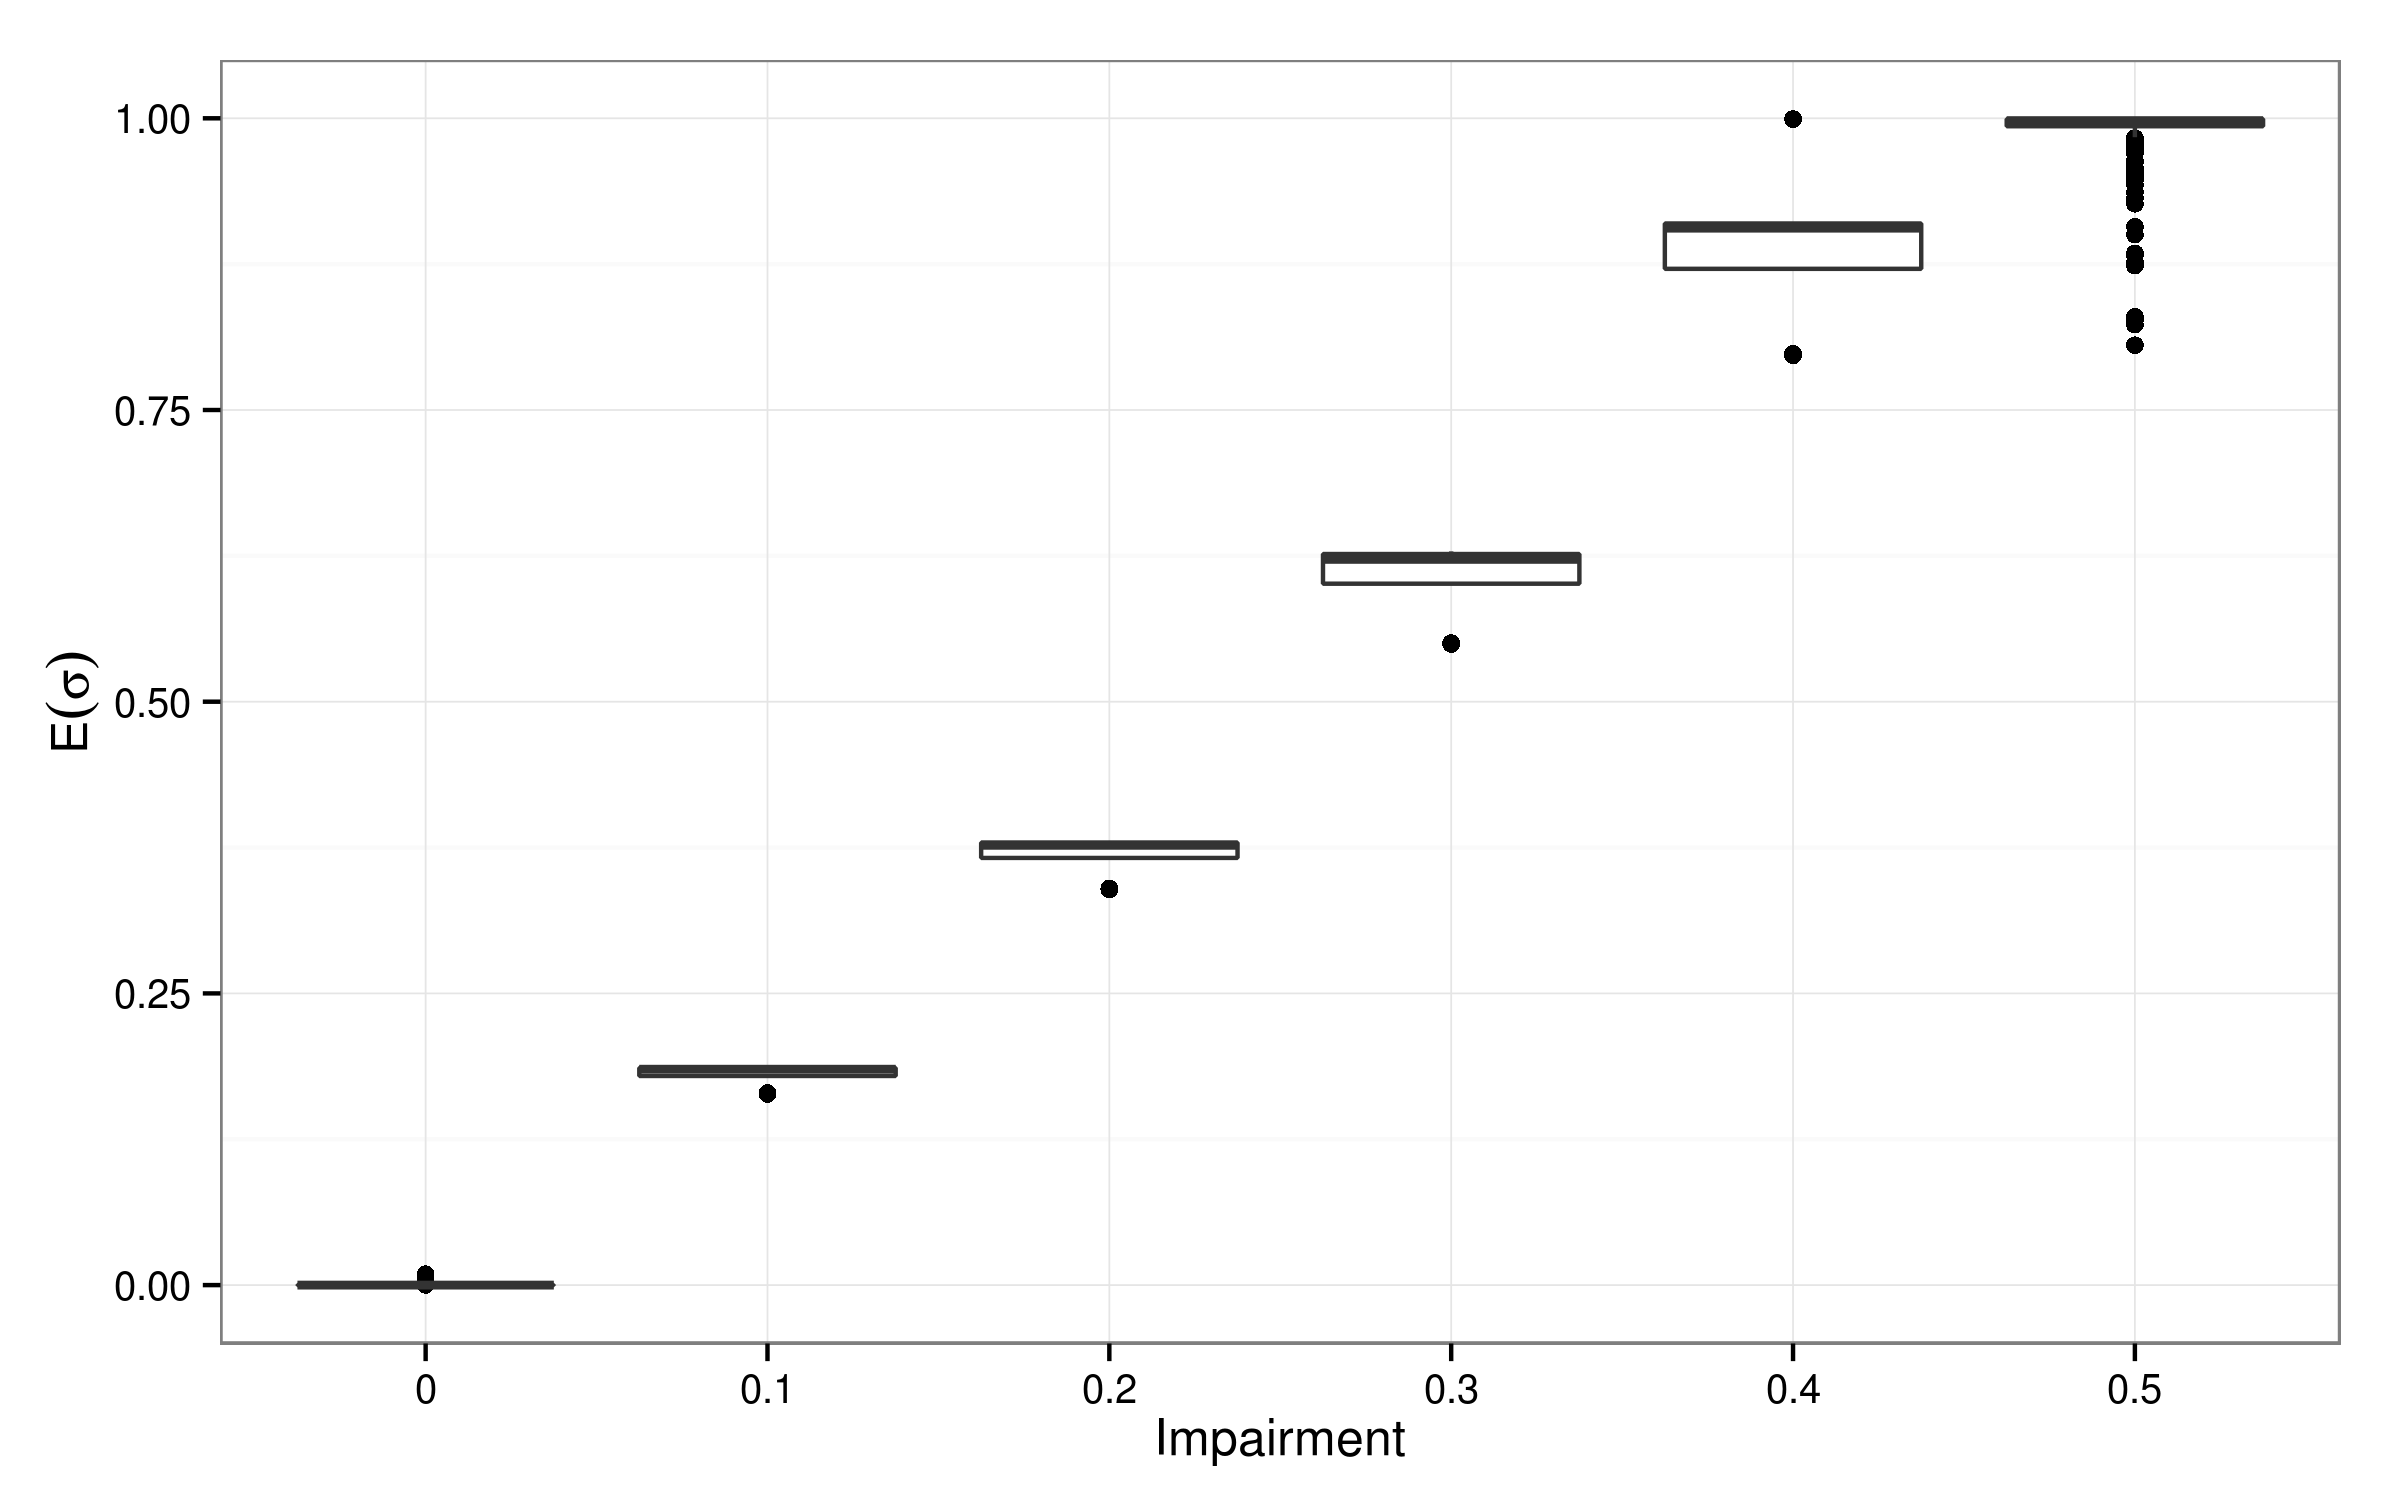
\includegraphics[width=\textwidth]{plots/Speaker-entropy-20140813-194306}
                \caption{Entropy of sender strategy.}
%                \label{fig:gull}
        \end{subfigure}
        \begin{subfigure}{0.45\textwidth}
                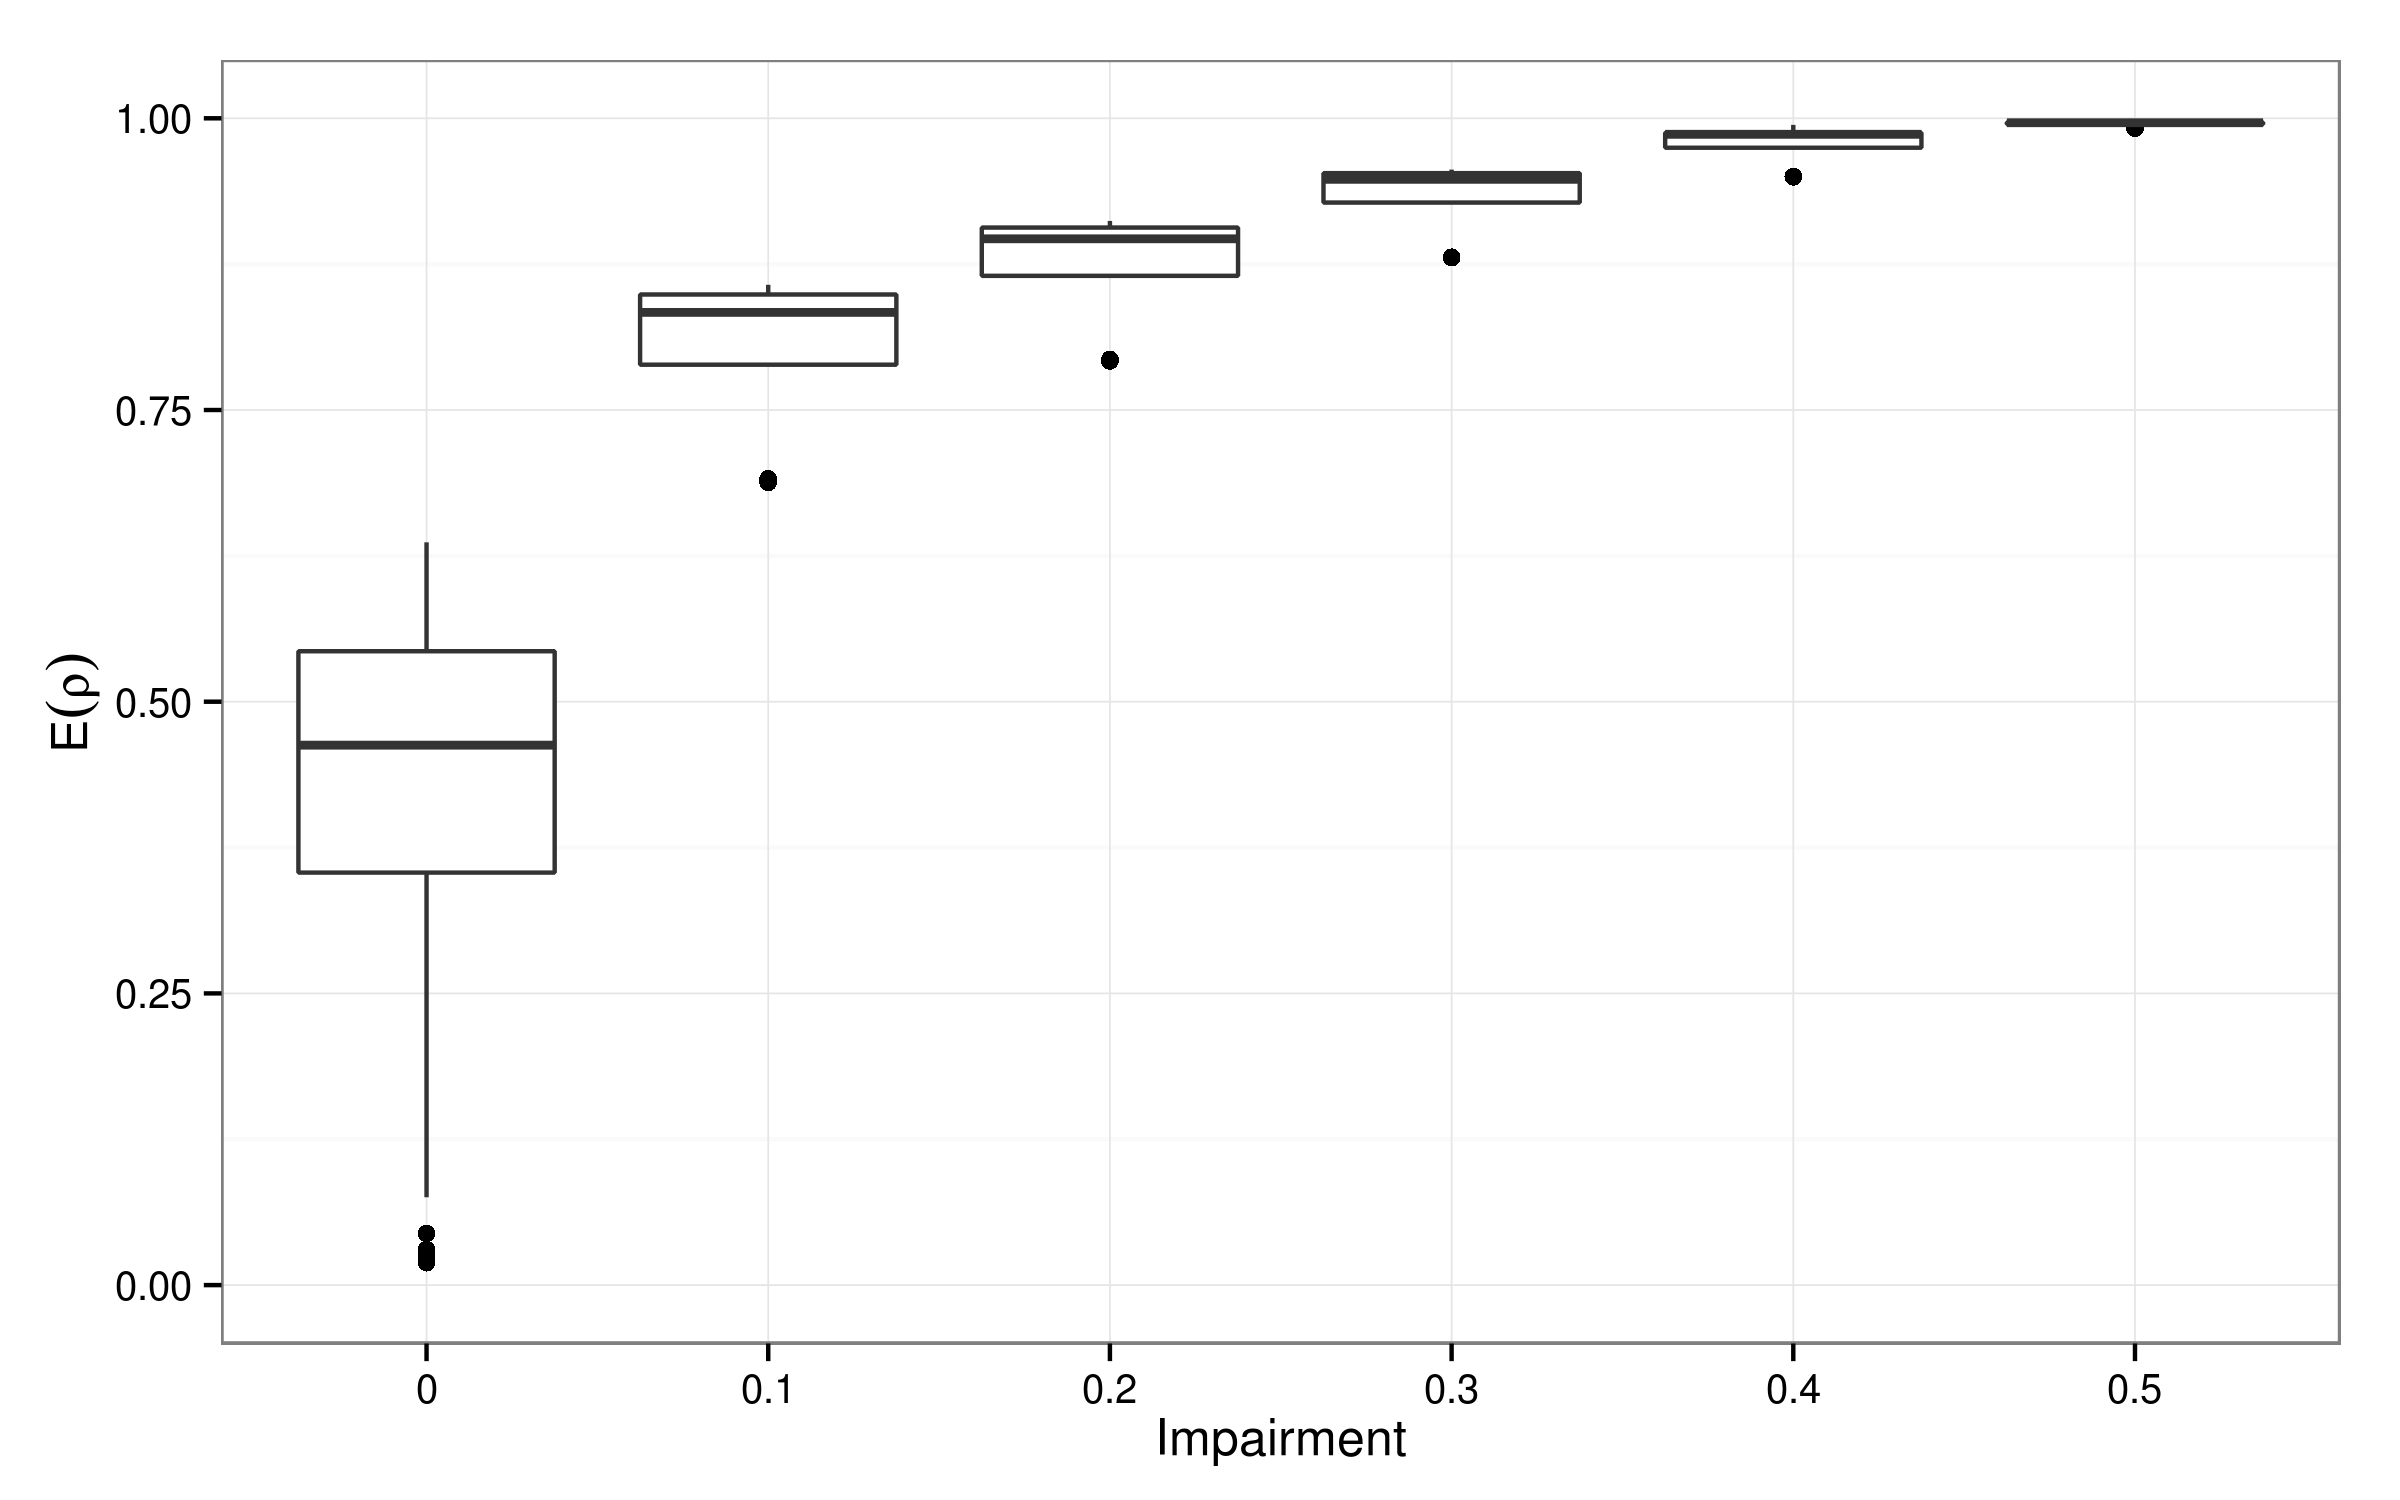
\includegraphics[width=\textwidth]{plots/Hearer-entropy-20140813-194306}
                \caption{Entropy of receiver strategy.}
        \end{subfigure}

        \begin{subfigure}{0.45\textwidth}
                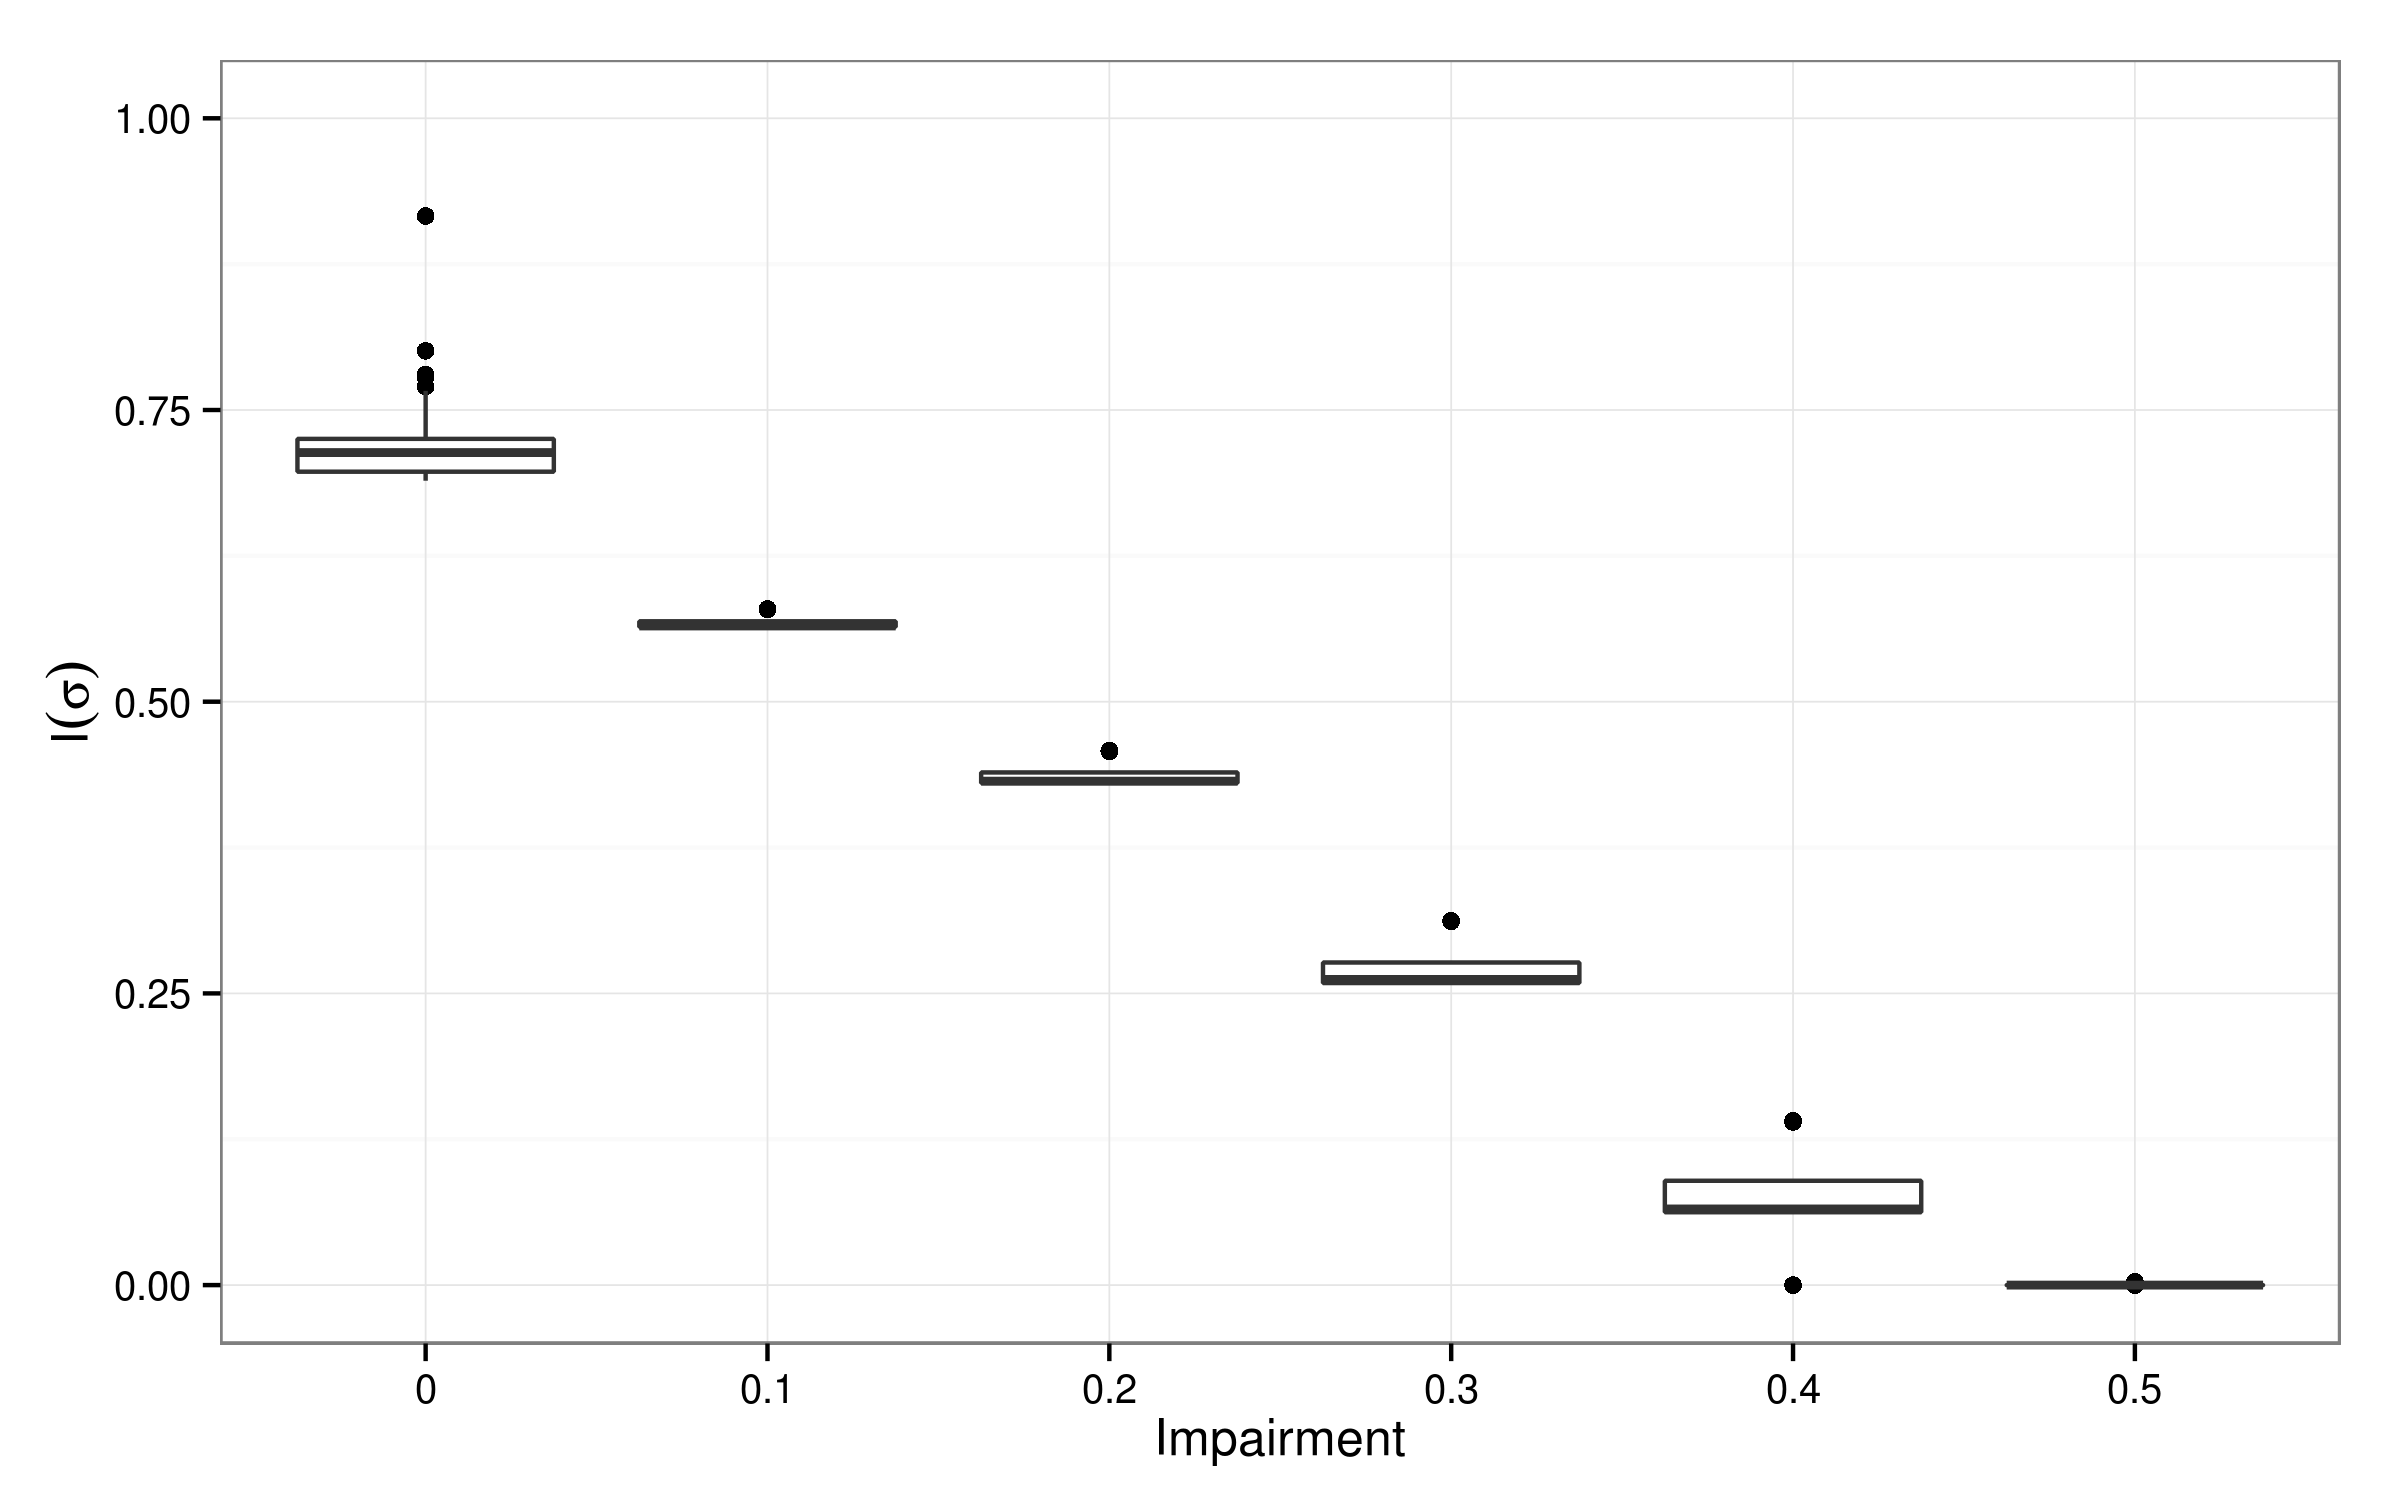
\includegraphics[width=\textwidth]{plots/Speaker-informativity-20140813-194306}
                \caption{Informativity of sender strategy.}
        \end{subfigure}
        \begin{subfigure}{0.45\textwidth}
                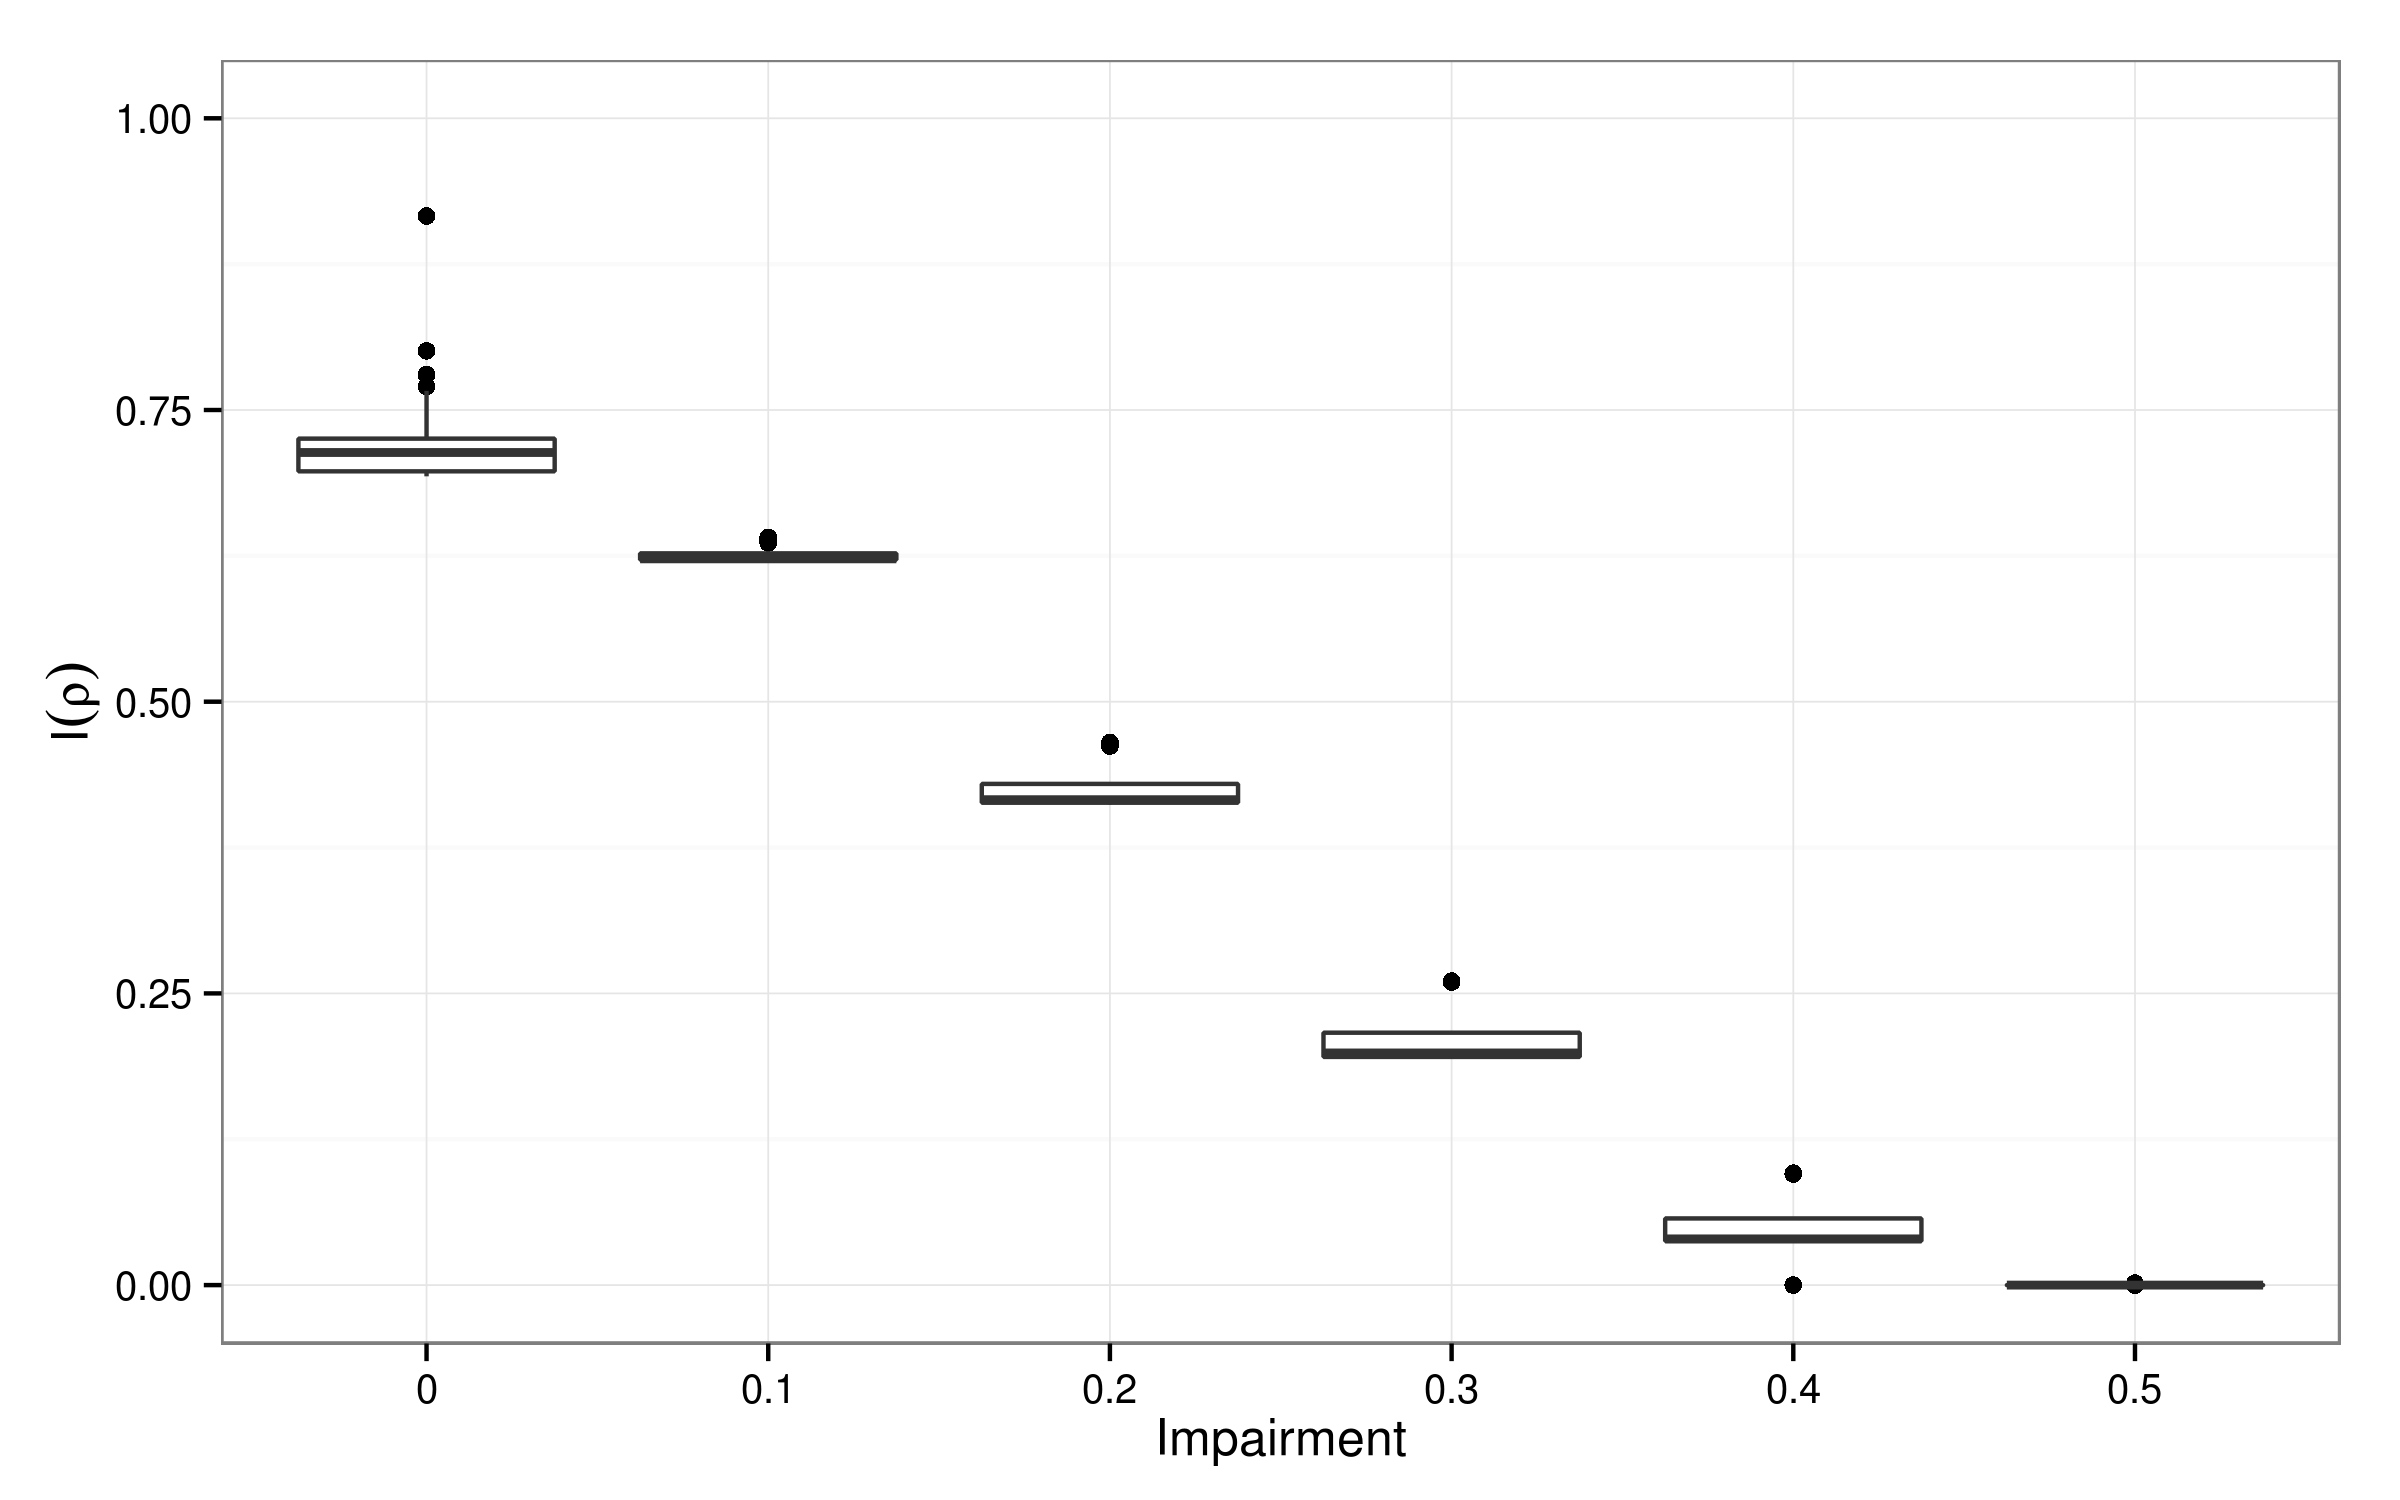
\includegraphics[width=\textwidth]{plots/Hearer-informativity-20140813-194306}
                \caption{Informativity of receiver strategy.}
        \end{subfigure}

        \begin{subfigure}{0.45\textwidth}
                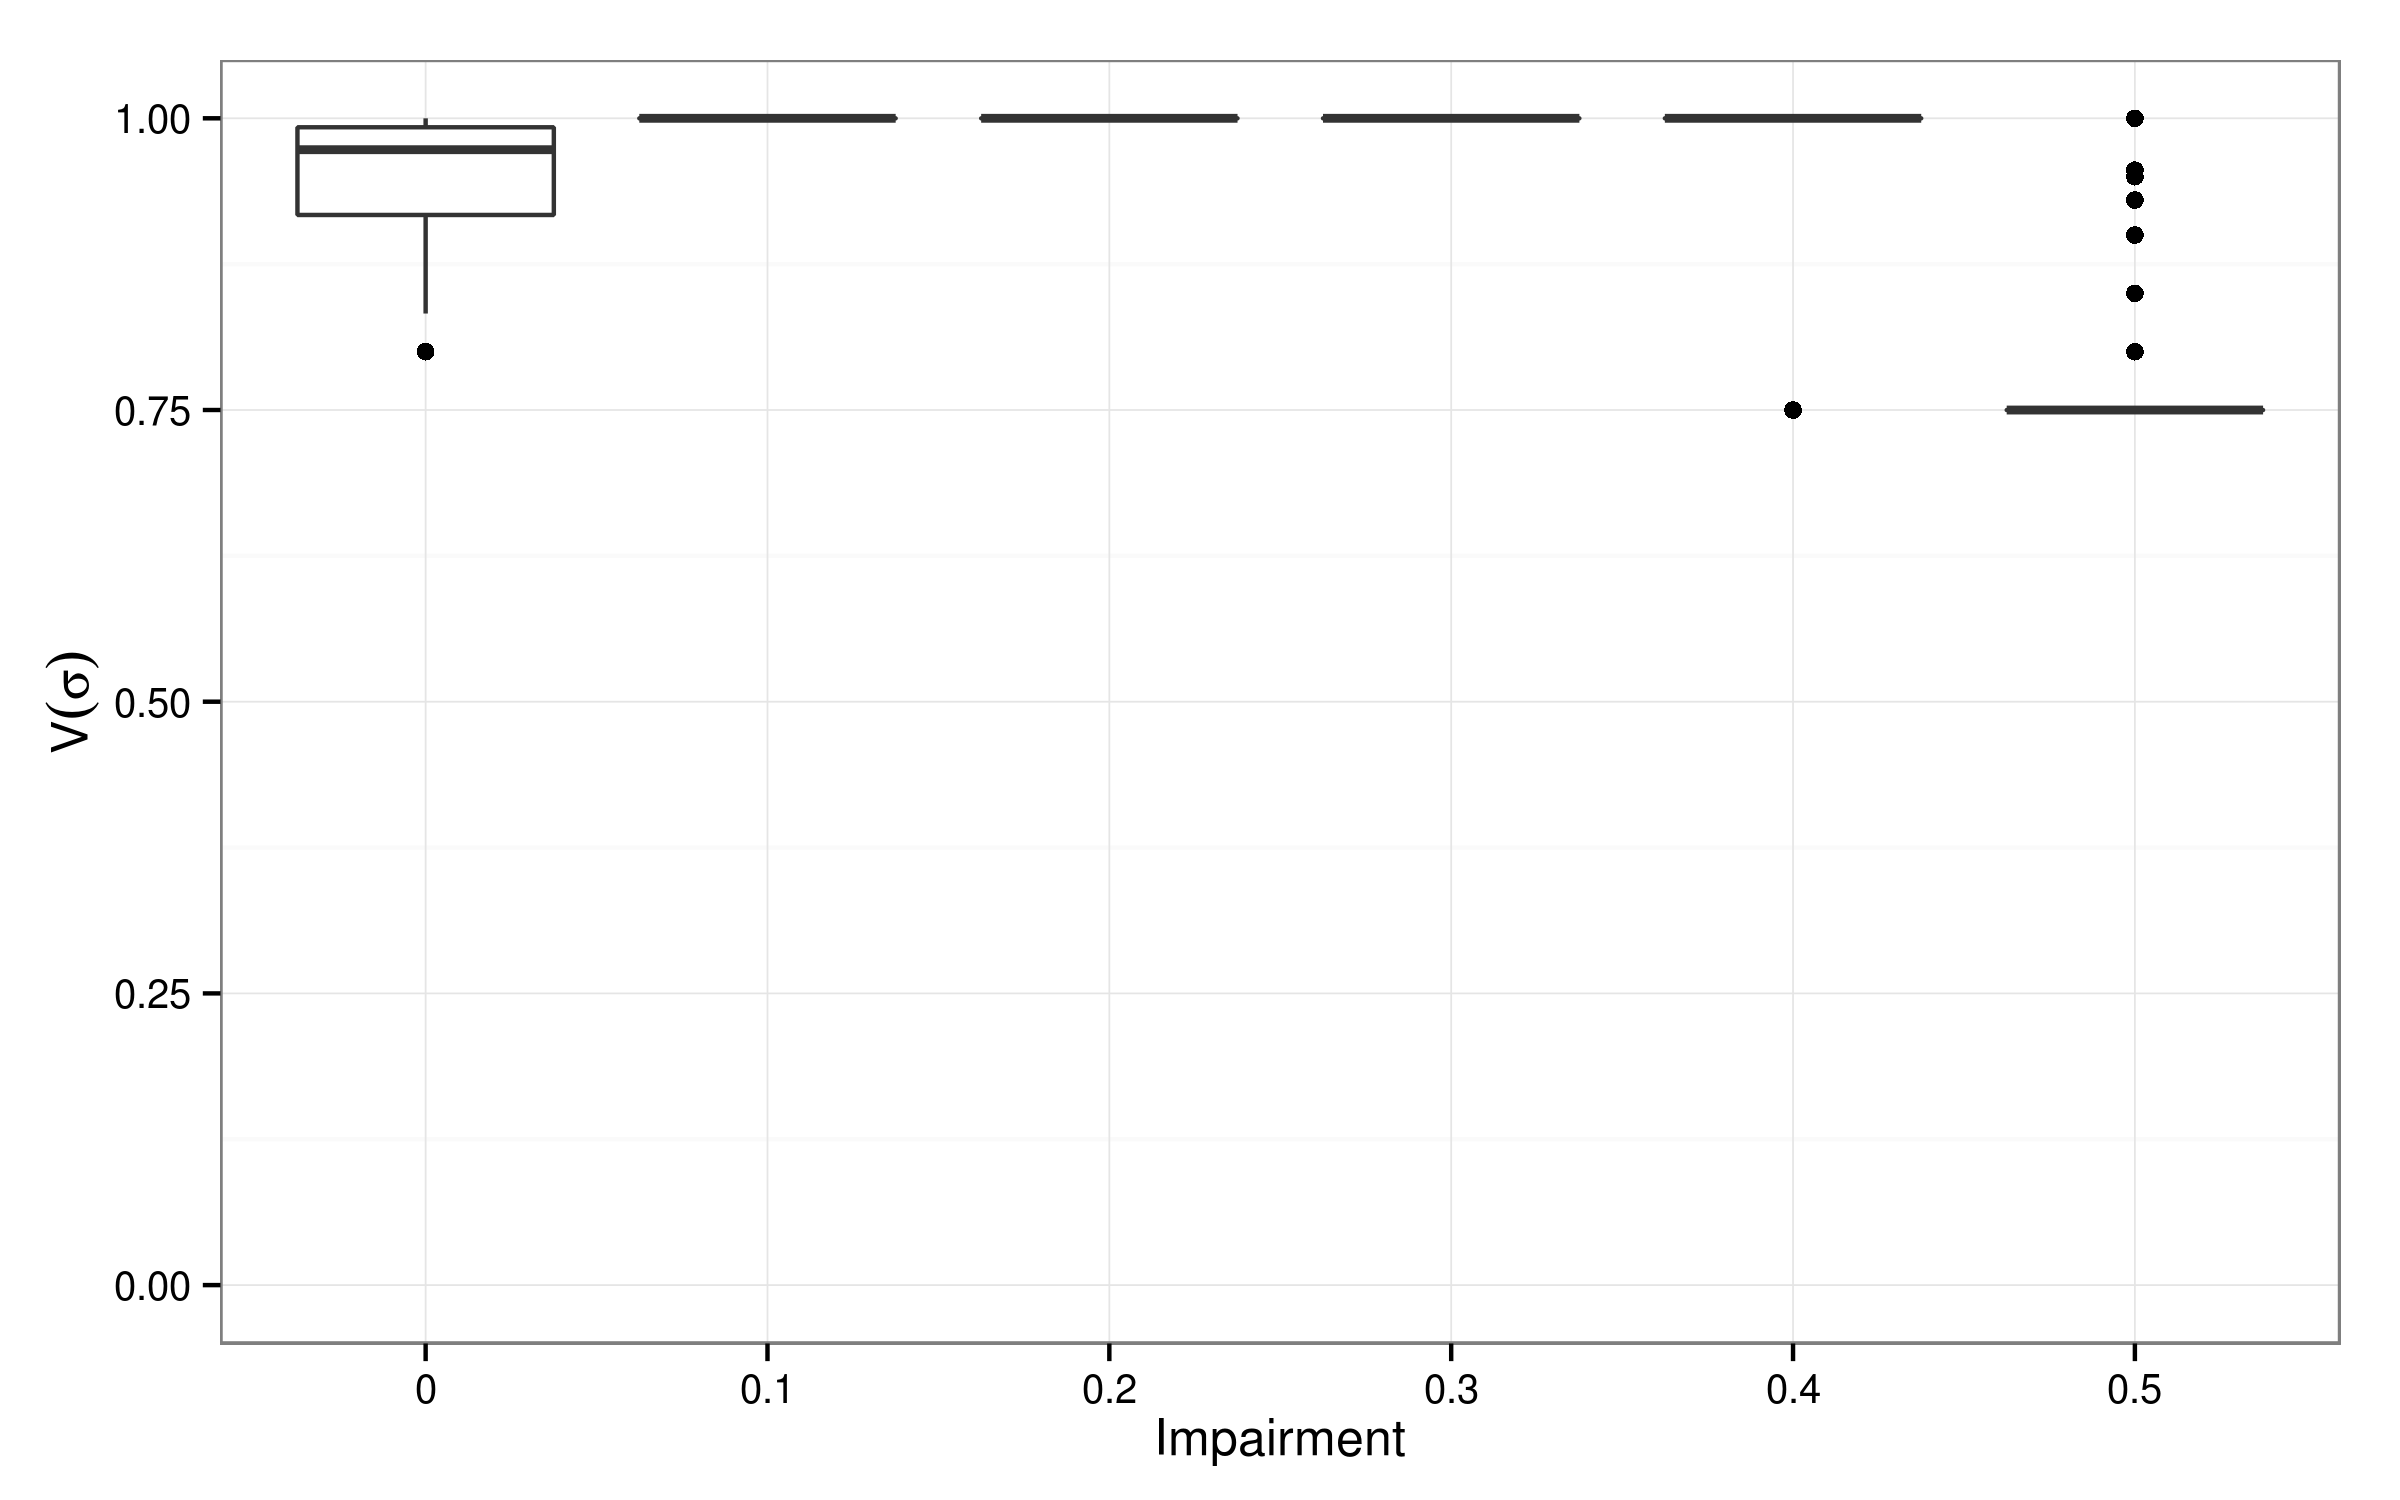
\includegraphics[width=\textwidth]{plots/Speaker-Voronoiness-20140813-194306}
                \caption{Voronoiness of sender strategy.}
        \end{subfigure}
        \begin{subfigure}{0.45\textwidth}
                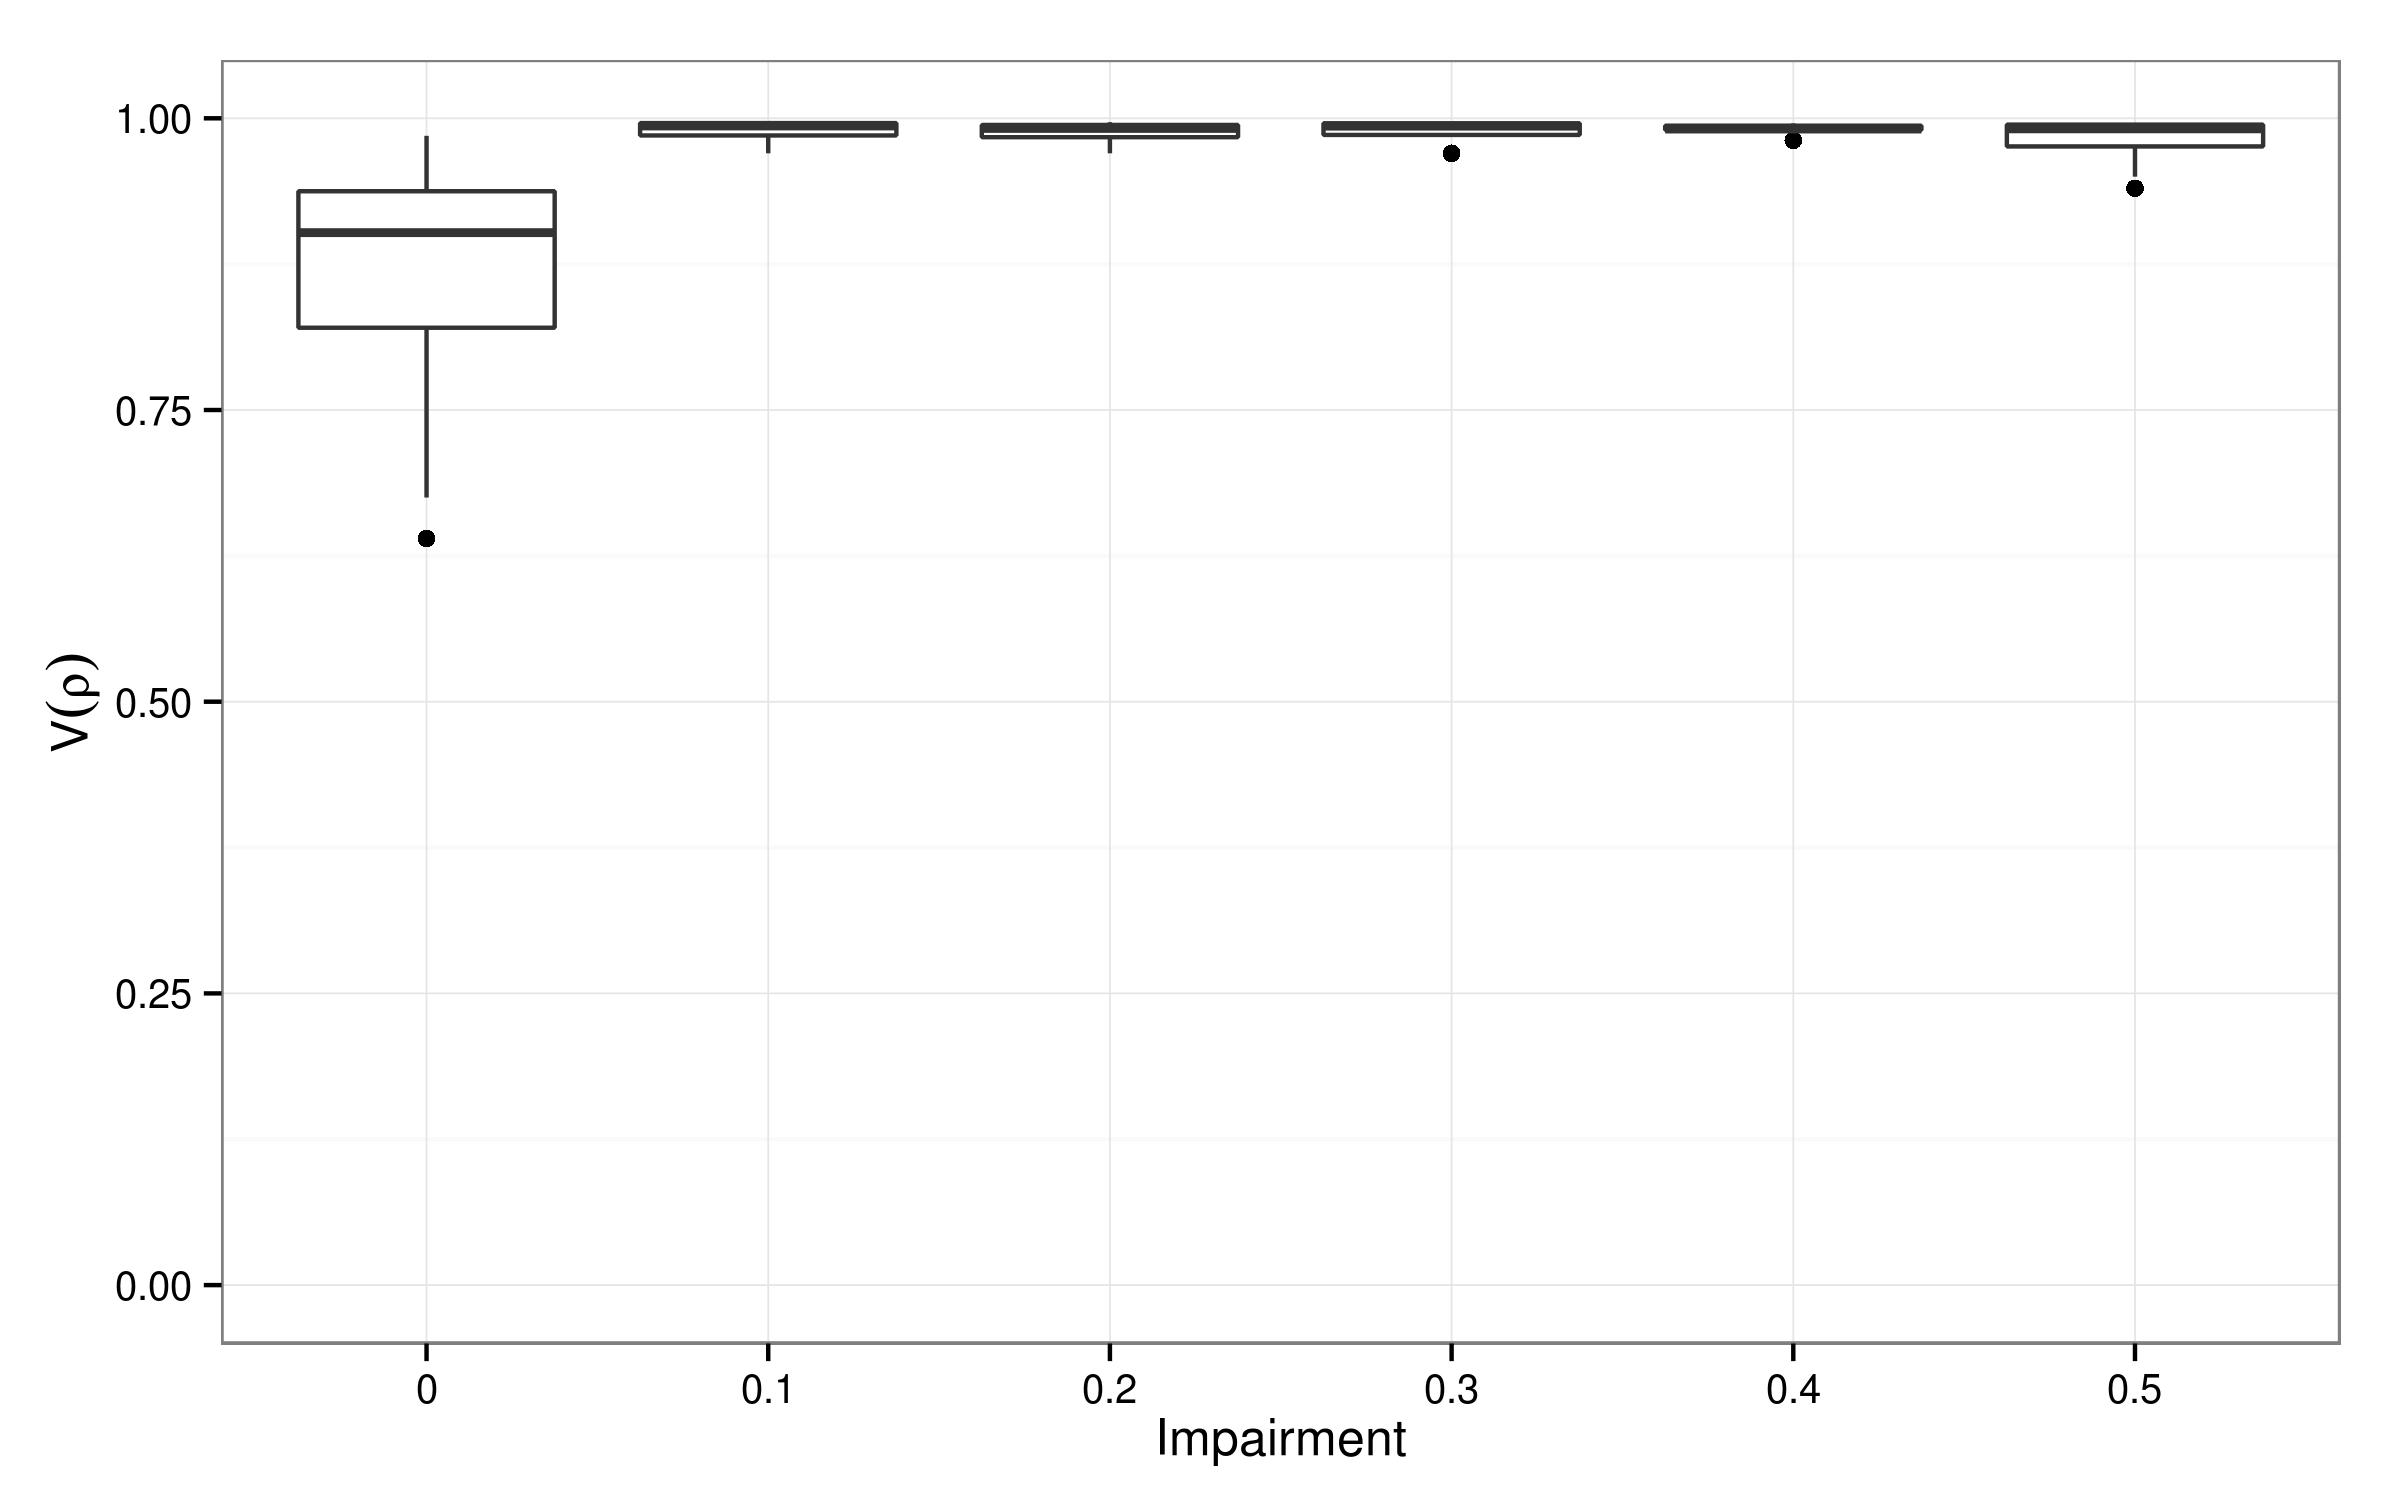
\includegraphics[width=\textwidth]{plots/Hearer-Voronoiness-20140813-194306}
                \caption{Voronoiness of receiver strategy.}
        \end{subfigure}

        \begin{subfigure}{0.45\textwidth}
                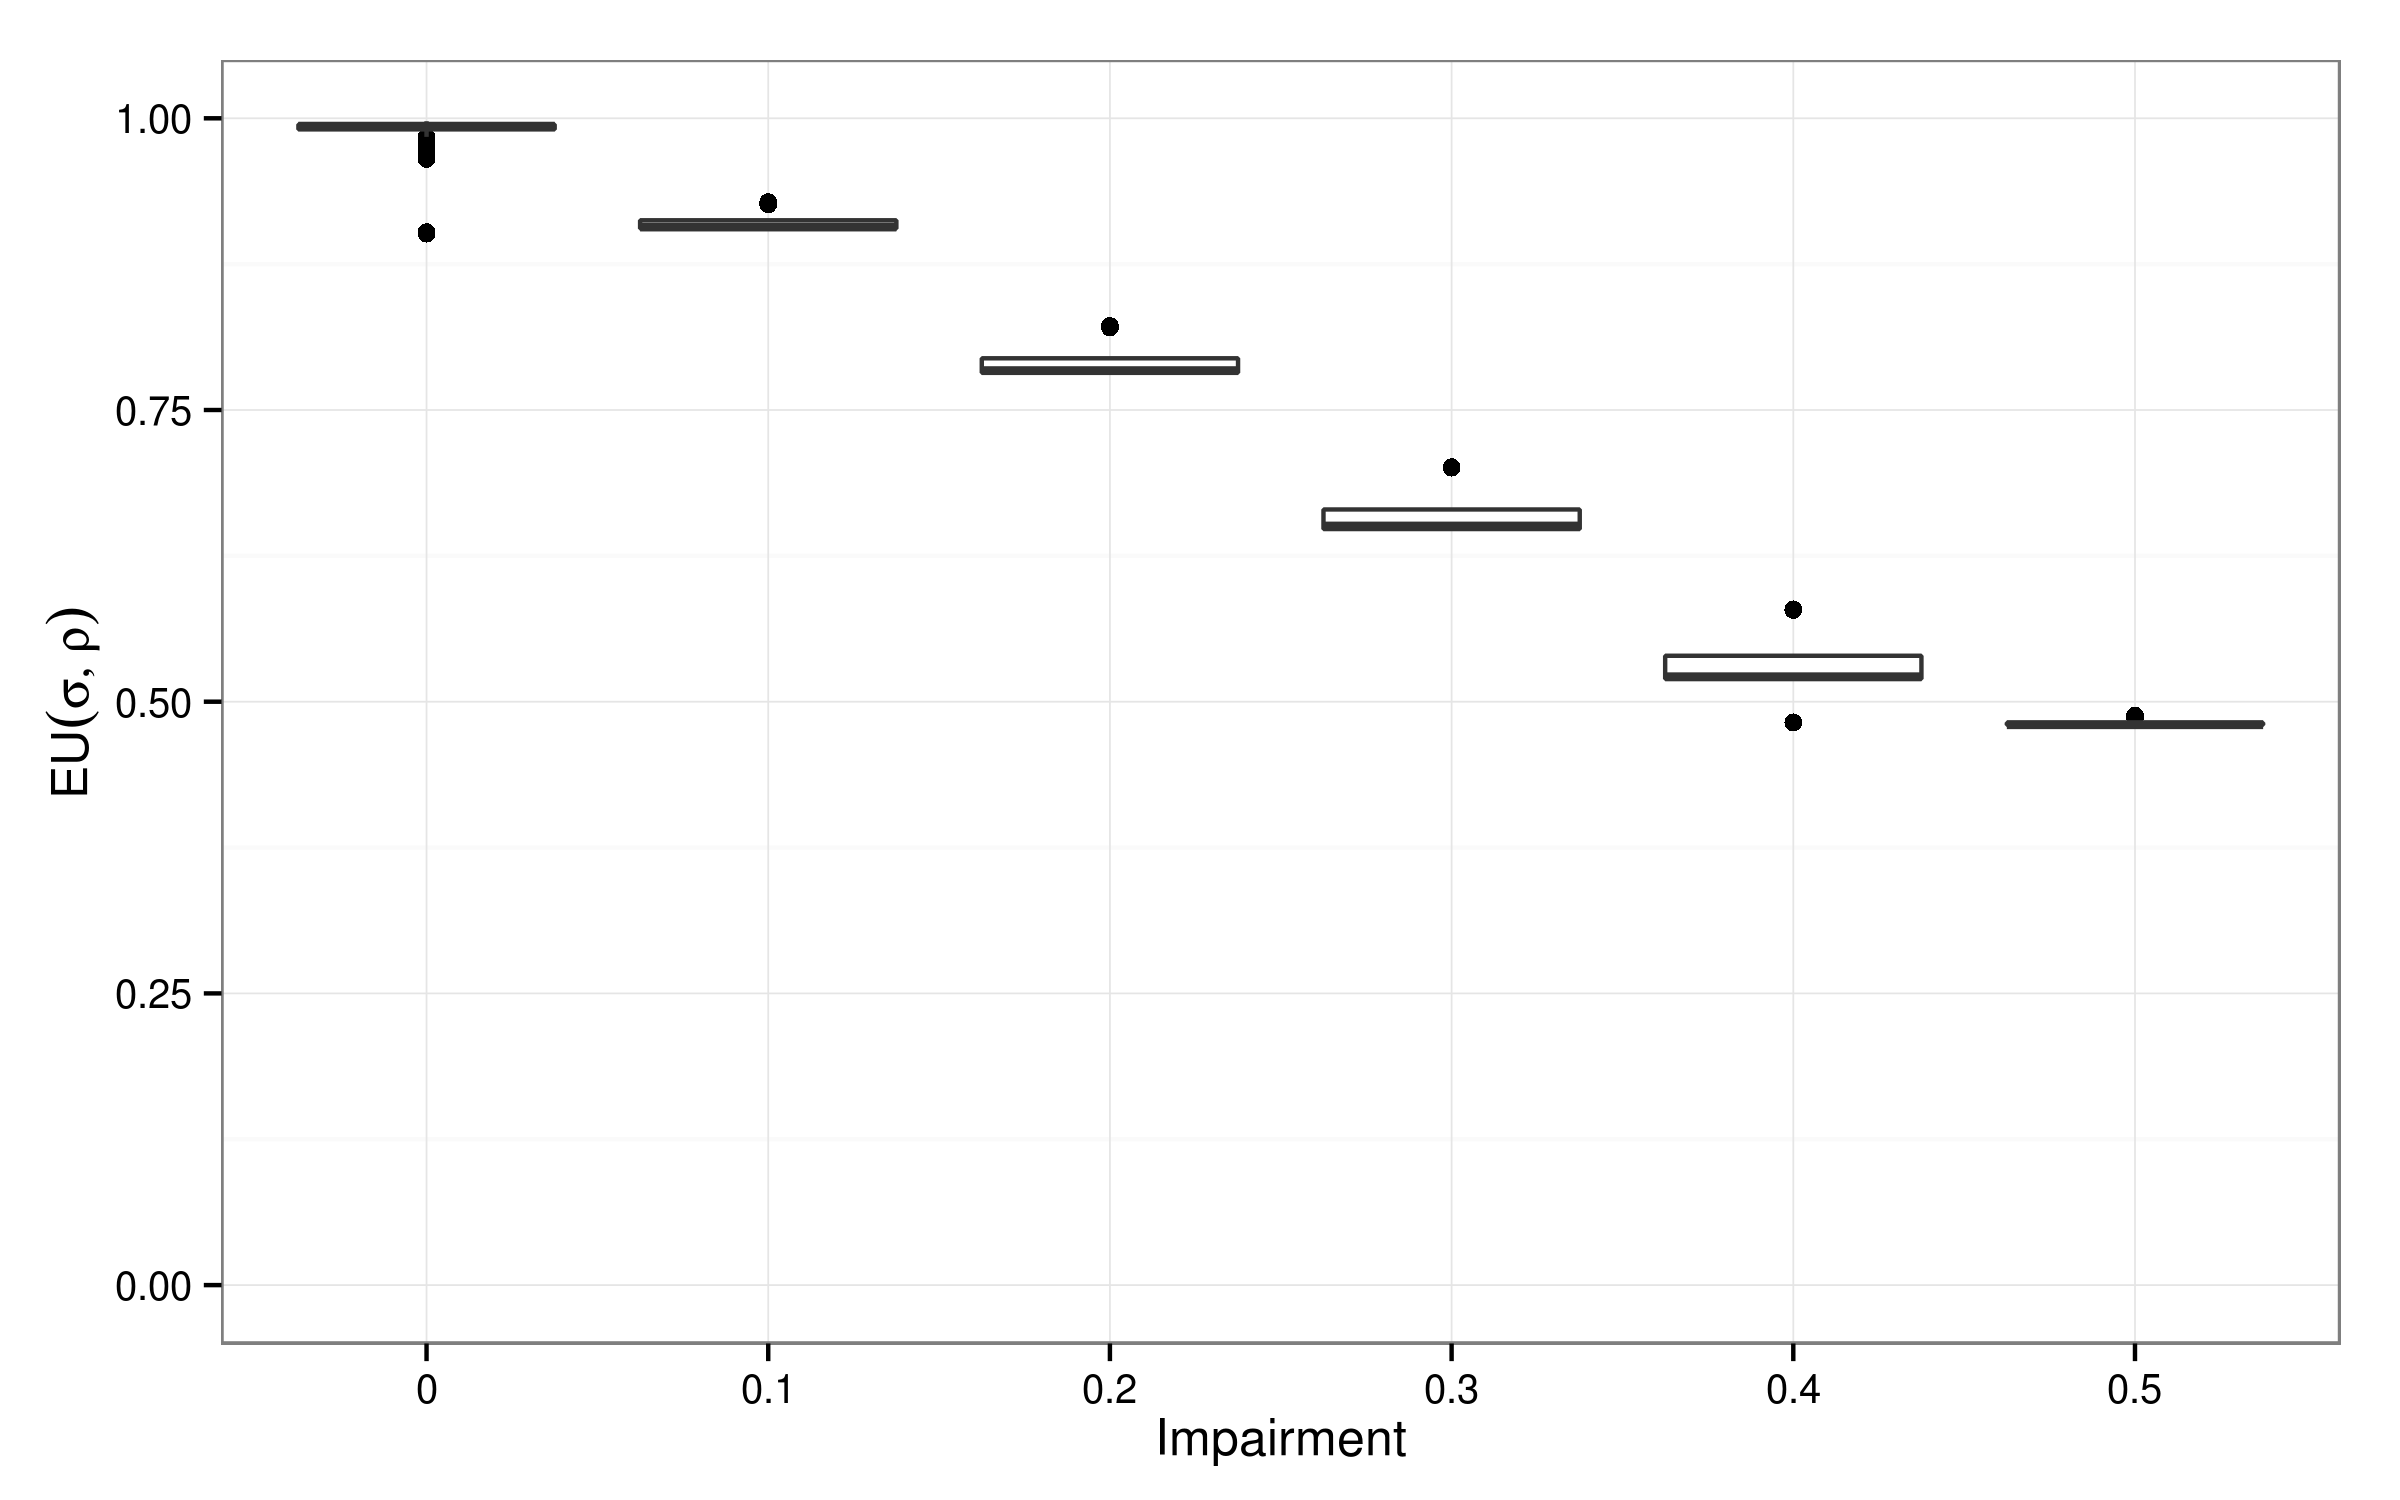
\includegraphics[width=\textwidth]{plots/Expected-utility-20140813-194306}
                \caption{Expected utility.}
        \end{subfigure}
        \begin{subfigure}{0.45\textwidth}
                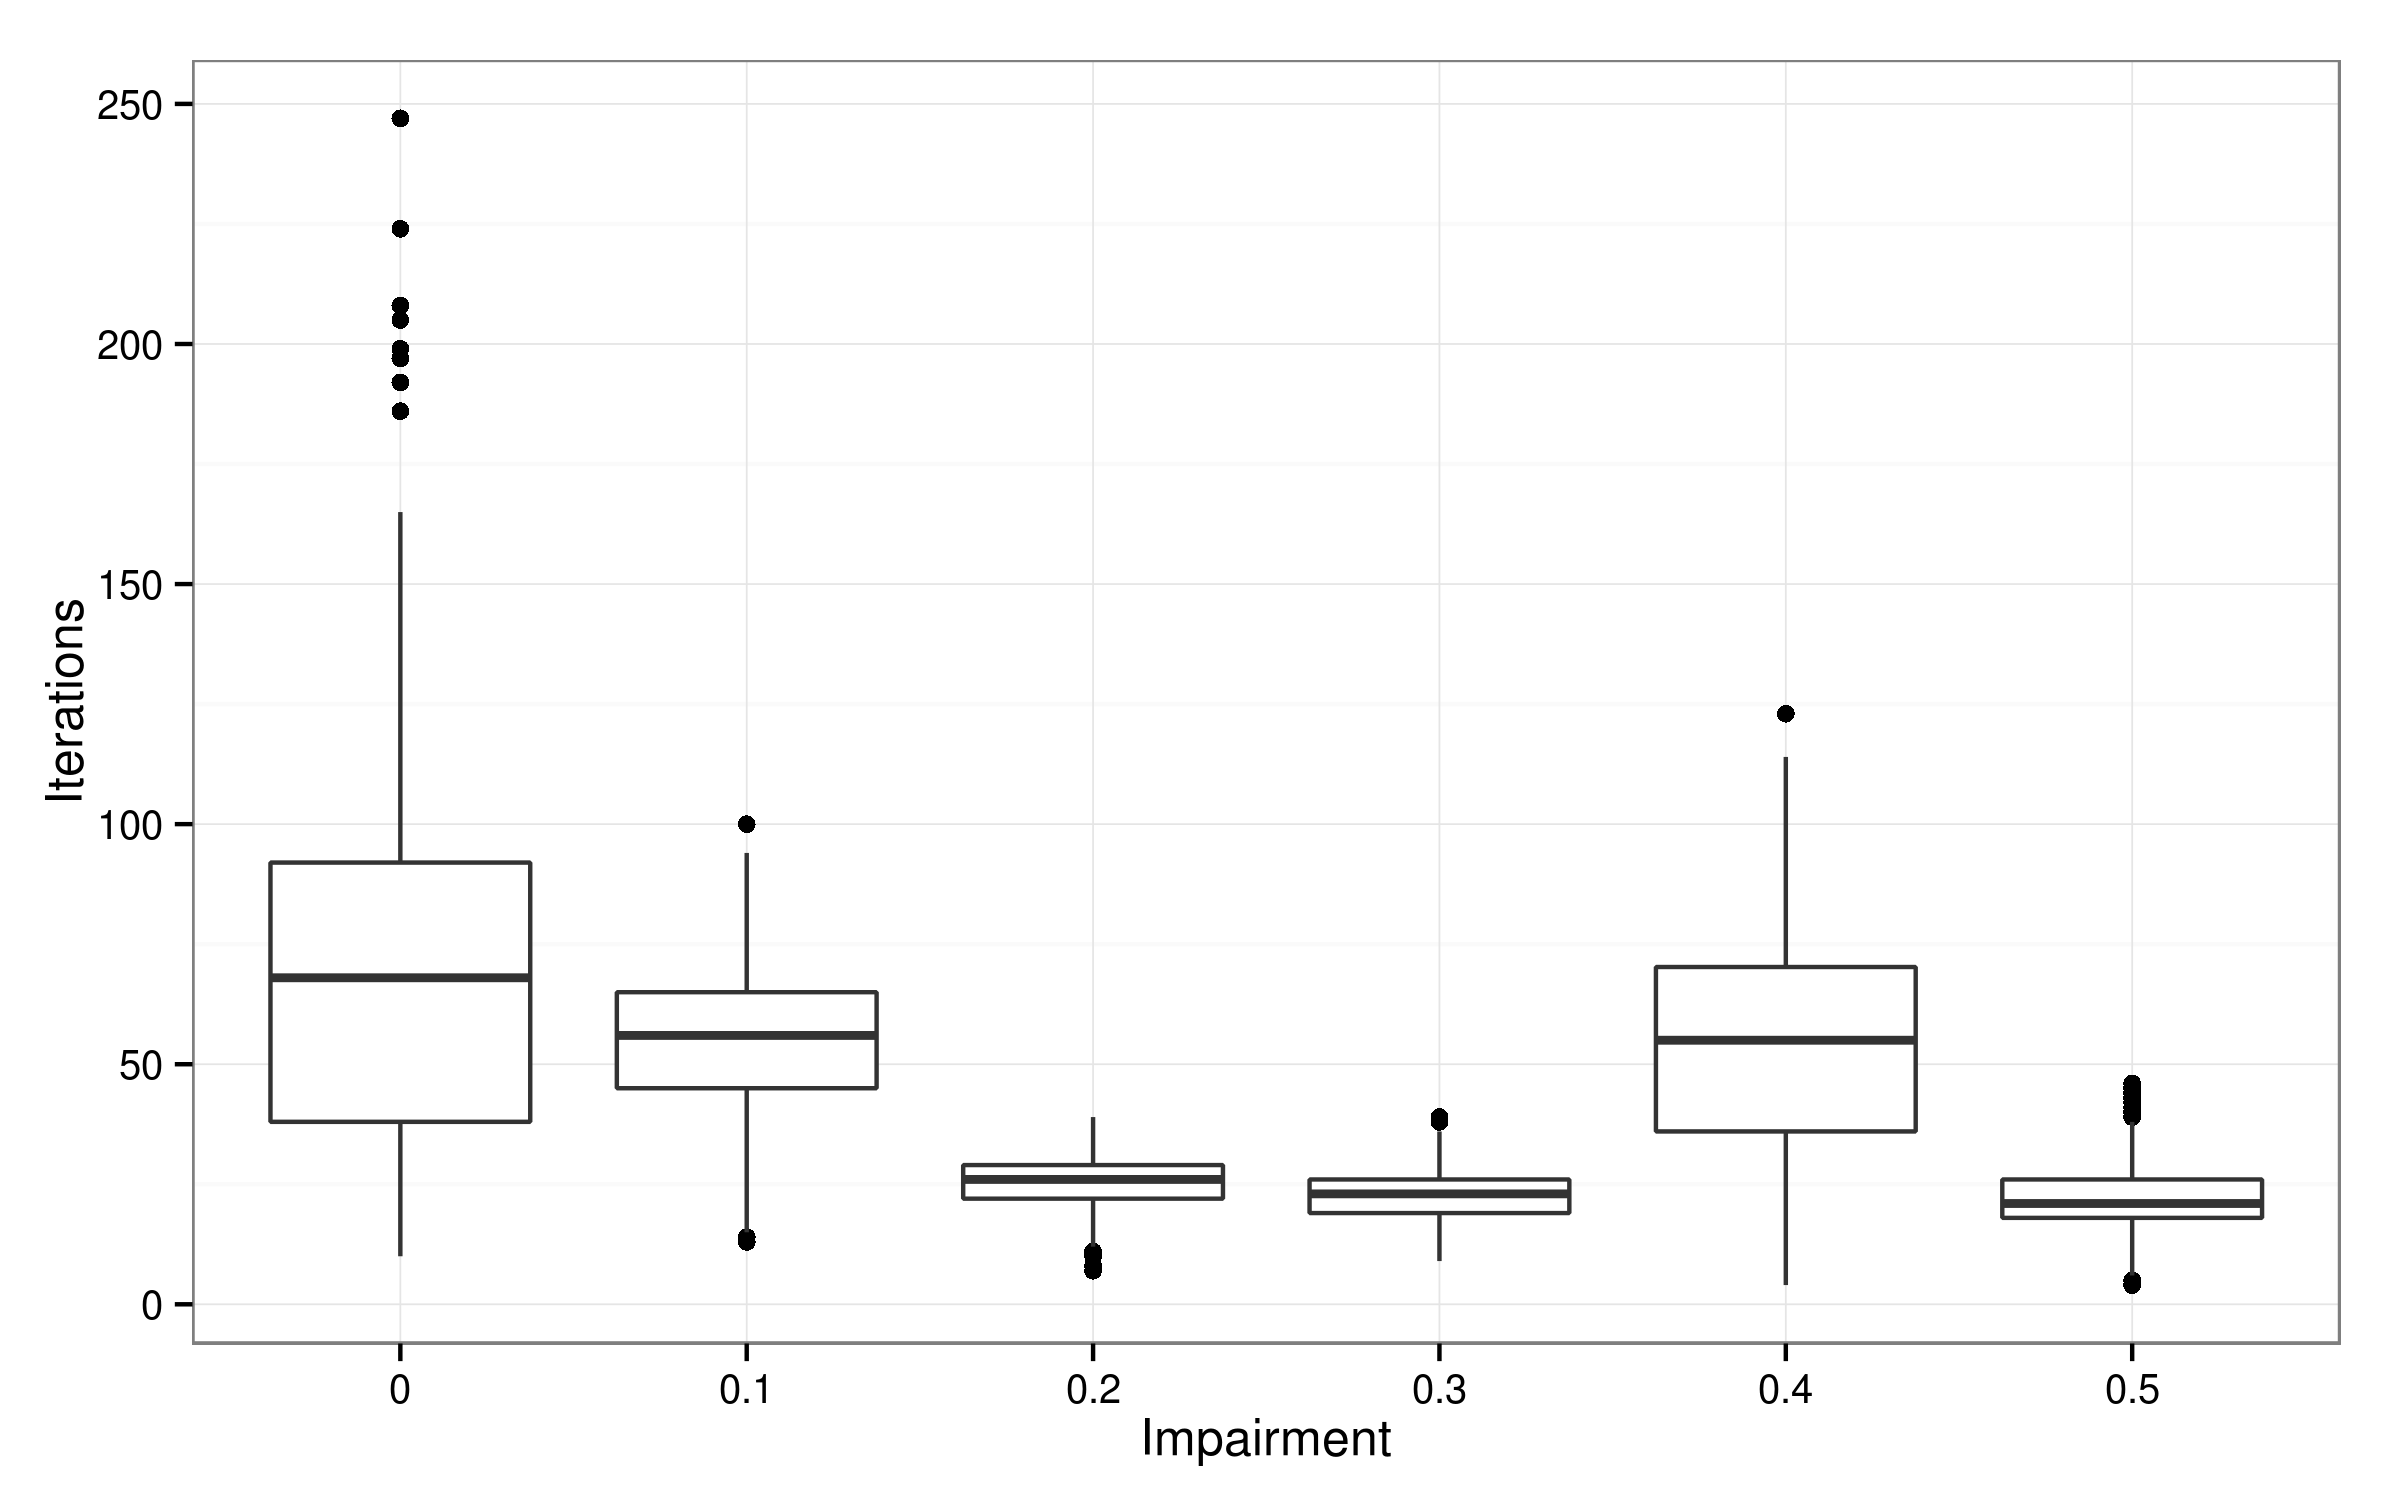
\includegraphics[width=\textwidth]{plots/Iterations-20140813-194306}
                \caption{Number of iterations until convergence.}
        \end{subfigure}
        \caption{Boxplots of metrics per impairment value.}
        \label{fig:metrics-boxplots}
\end{figure}
%
Most trends are quite clear.
Entropy seems to increase with higher impairment values for both sender and receiver.
This is an expected outcome, since the higher the impairment value, the more likely each player is to confuse two states, thus the more uncertain he will be in unequivocally associating a state with a message, or vice-versa.
The trend for informativity is also expected: more vague strategies convey less information, be it from the sender or the receiver perspective.

Regarding Voronoiness, we observe that most simulation results approximate perfect Voronoi tessalations.
This is not the case, however, for impairment of $0$ (both sender and receiver) and $0.5$ (mostly sender only).
\mytodo{JPC}{For impairment 0, the languages with the lowest sender voronoiness look like non-convex equilibria. Discuss in relation with Elliott's results?}
For impairment of $0$,  the explanation is usually that strategies can achieve a high expected utility without having perfect Voronoiness.
Although the expected long term outcome in these situations is perfect Voronoiness (given J\"ager's analytical results~\cite{Jager2007}), actually reaching it involves minor refinements which at some point do not qualify as significant change given our convergence criterion.
The result is thus an artifact of stopping the simulations before they reach perfect convergence.
For impairment of $0.5$ (and some cases with impairment of $0.4$), the reason is simply that the languages are representatives of something between babbling and pooling equilibria.
These are equilibria where $\Sstrat(\state,\messg_1) \geq \Sstrat(\state,\messg_2)$ for all $\state \in \States$, but vary from situations where $\Sstrat(\state,\messg)$ is close to $0.5$ for both messages (babbling), or is significantly higher for one of them (pooling).
\mytodo{JPC}{Plot examples}

The trend for expected utility reflects Lipman's observation that vague languages are less optimal than non-vague ones~\cite{Lipman2009:Why-is-Language}: more impairment necessarily leads to lower expected utility.
Finally, the plot for number of iterations until convergence shows that a certain level of impairment enables faster convergence.
We will discuss this further in more detail in Section~\ref{sec:discussion}.

\mytodo{JPC}{Present and discuss results per size of state space? Don't forget O'Connor's claim that speed of convergence is more important for larger \#state/\#message ratio}


%%% Local Variables: 
%%% mode: latex
%%% TeX-master: "paper"
%%% TeX-PDF-mode: t
%%% End:





\section{Discussion}
\label{sec:discussion}

We have introduced a new variant of the replicator mutator dynamics
that implements specifically stochastic noise in the form of
confusability of similar states. The probabilities of confusing nearby
similar states is easily implemented in behavioral strategies, but can
also be translated into a mutation matrix for pure strategies. This
allows, in principle, several conceptual interpretations of the \rdd,
on which we will briefly enlarge below in
Section~\ref{sec:model-interpretation}.

Next to this technical contribution, the results of our numerical
simulations also advance our understanding of the possibility of
evolving regular and efficient categories despite their (higher-order)
vagueness. Section~\ref{sec:relat-with-prev} zooms in on the relation
with closely related accounts once more, to delineate the present
approach more precisely.

\subsection{Model interpretation}
\label{sec:model-interpretation}

We mentioned in passing in Section~\ref{sec:repl-diff-dynam-1} that
adding diffusion to other discrete-time evolutionary dynamics that
operate on behavioral strategies is entirely straightforward. We
could, for instance, easily diffuse the outcome of a best-response
dynamic at each time step. That would make sense if we thought of
agents as prone to confusing similar states that are otherwise
rational optimizers of behavior. The reason that we chose the
replicator dynamics to combine with diffusion is twofold. A minor
reason is that it makes for a conceptually interesting link with the
replicator mutator dynamics. A more important reason is that the
replicator dynamic is especially versatile and non-committal about
what the exact process of adaption is that is being modelled.

Originally the \rd was introduced as mathematical model of evolution
under asexual reproduction, motivated by concepts from the theory of
natural selection \citep{TaylorJonker1978:Evolutionary-St}. The most
conservative interpretation of the \rdd in our present context is thus
a biological one: we can imagine signaling strategies as innate or
fixed behaviorial tendencies of organisms, steps in the evolutionary
process as successive generations, and selection as capturing the
reproductive advantage of fitter individuals. This interpretation,
strictly speaking, requires formalization in terms of mixed strategies
via the \rmd, and possibly also a symmetrizing of the game, so that
every agent is assumed to have a unique sender and receiver role at
the same time the is bequeathed onto the next generation. Diffusion,
in this context, could be either of two things. It could be
differential mutation probabilities in line with other interpretation
of mutation in the \rmd
\citep[e.g.][]{NowakKomarova2001:Evolution-of-Un,KomarovaNiyogi2001:The-Evolutionar}:
pure strategies are not faithfully reproduced, and mistakes in
bequeathing pure strategies are more likely if they result from the
confusion of similar states. Another possible biological
interpretation of the \rdd, is that inheritance is faithful, but
strategies are noisily realized. Strategies are not necessarily
selected for what they are, but rather for how they are realized, once
noise is factored in. 

But the replicator dynamic is not only a model of biological
evolution. It can also be interpreted as a high-level description of
the likely development of other behavioral adaptation processes, like
differential imitation and cultural evolution in general
\citep[see][for various derivations of the
\rd]{Sandholm2013:Population-Game}. Under this interpretation, the \rd
is consistent with the idea that what is subject to the evolutionary
forces are not organisms but behavior: individuals can adapt their
behavior to the perceived environment or adopt strategies from other
individuals. Fitness captures the success of behavioral patterns,
which in the case of language can be thought of in terms of
communicative success.  Differential reproduction represents the
tendency of more successful strategies to be more likely adopted by
individuals, be it through imitation or some learning procedure within
the population.  

Under this non-biological interpretation, we have again two options of
picturing what diffusion is, similar to the biological cases
before. One possibility is that diffusion is noise in the adoption of
strategies, say, by conditional imitation, of strategies by other
signalers. Another possibility is that diffusion is again noise on the
realization of strategies: while behavior is optimized to be efficient
(be it due to learning, introspection or imitation), realization of
strategies is bound to be noisy due to confusability of similar
states. 

We believe that all of the four mentioned interpretations are, on
first approximations, feasible conceptualizations of the \rdd, and
that it is a good thing to know of a working account of vague
signaling that sketches where fitness-based selection under
state-confusability will take is, abstracting away from the details of
actually playing the game, inheriting, imitating or otherwise
optimizing behavior in whatever particular way. It is a good thing to
know this on the macro-level, especially since there are also
micro-level accounts that nicely complement the picture. We turn to
one such next.


\subsection{Relation with previous accounts}
\label{sec:relat-with-prev}

\paragraph{Generalized reinforcement.}
\citet{OConnor2013:The-Evolution-o} introduces a generalization of
Herrnstein reinforcement learning for sim-max games and showed that
this not only leads to vague signaling patterns, but can speed-up
evolution of efficient signaling strategies, especially in games with
many states. 

Under plain Herrnstein reinforcement learning, sender and receiver
play the game repeatedly and adjust their dispositions to act after
each round of play, in such a way that the actual (non-negative)
payoff gained in the current interaction is added to the
non-normalized propensities for acting in exactly the way that they
acted in the current round of play. For sim-max games, this means that
when the sender chose $\messg$ in state $\state$, and this resulted in
some non-negative payoff (which is guaranteed by our choice of utility
function), the probability that the sender chooses $\messg$ again in
$\state$ is increased, but nothing else changes. In particular, the
speakers behavior in other choice points does not change. Generalized
reinforcement learning is different here. When the use of $\messg$ in
$\state$ gave positive payoff, then not only will its future use
probability be promoted at $\state$ but also at other states,
proportional to how similar these are to $\state$. Similar amendments
take care of the way that the receiver updates his choice
dispositions.

\citet{OConnor2013:The-Evolution-o} shows that this extension not only
leads to vague signaling of the appropriate kind, but also speeds up
learning in such a way that, especially for games with higher numbers
of states, higher levels of communicative success are reached in
shorter learning periods than is possible without stimulus
generalization. Technically, this result is partly due to the fact
that signalers make bigger changes to their behavioral strategies
after each round of play under generalized reinforcement than under
the plain variety. But that only explains the speed of adaptation, not
necessarily that generalization also leads to regularity and
communicative efficiency. 

Diffusion of strategies in the \rdd can be conceived of as a form of
generalization as well, and works in large part quite analogous to
stimulus generalization in \citeauthor{OConnor2013:The-Evolution-o}'s
approach. This holds for the effect of diffusion and generalization,
but not necessarily for the way that the effect is achieved. We also
saw that diffusion in \rdd leads to more regular languages and
speedier convergence. However, the \rdd is a more abstract framework
than generalized reinforcement learning. The latter is foremost
motivated as a learning dynamic that has two players adapt their
individual strategies after each concrete round of play. In contrast,
the \rdd describes a more abstract, average dynamical change in
behavioral dispositions. Although the dynamics of (some forms of)
reinforcement learning mirror those of the replicator dynamics (at
some stage in time)
(\cite{BorgersSarin997:Learning-Throug,HopkinsPosch2005:Attainability-o,Beggs2005:On-the-Converge}),
this does not mean that \emph{generalized} reinforcement learning, in
which stimulus generalization is best motivated at the level of a
single agent's dispositional generalization after one round of play,
is also directly a plausible high-level description of, say,
generalized learning in a population of agents. Seen in this light,
generalized reinforcement learning and the \rdd nicely complement each
other, as similarly-minded accounts operating at different levels of
abstraction.

\paragraph{Quantal response equilibria.}
\citet{FrankeJager2010:Vagueness-Signa} suggested a number of ways in
which information processing limitations of signaling agents could
lead to vague strategies. The model that is most clearly related to
the present approach uses the notion of a quantal response, also known
as a logit response or a soft-max function
\citep[e.g.][]{Luce1959:Individual-Choi,McFadden1976:Quantal-Choice-,McKelveyPalfrey1995:Quantal-Respons,McKelveyPalfrey1998:Quantal-Respons,GoereeHolt2008:Quantal-Respons}. A
quantal response function is a paramterized generalization of the
classic best response function. For example, if $U \mycolon \Acts
\rightarrow \mathds{R}$ is the measure of expected utility over
choices $\Acts$ of an agent, then a best response function would have
the agent choose $\act$ only if $U(\act) = \max_{\act' \in \Acts}
U(a)$. A quantal response function rather assumes that agents would
choose $\act$ with a probability proportional to $\expo(\lambda \cdot
U(\act))$, where $\lambda$ is a rationality parameter. If $\lambda
\rightarrow \infty$ we retrieve the behavior of the best response
choice function, but if it is positive but finite, any choice $\act$
will receive a positive probability, but acts with higher expected
utility will be more likely. The underlying motivation for this choice
rule is the assumption that there is noise in the computation of
expected utilities and/or in maximization of expected
utilities. Consequently, choices with almost equal expected utilities
will be chosen with almost equal probability (for moderate values of
$\lambda$). 

\citet{FrankeJager2010:Vagueness-Signa} show that quantal response
equilibria of sim-max games, i.e., pairs of sender and receiver
strategies such that the sender strategy is the quantal response to
the expected utilities under the receiver strategy and vice versa, can
show the desired marks of vague
signaling. Figure~\ref{fig:exampleQRE_stratsA} gives an example of a
quantal response equilibrium for a sim-max game, as used in our set-up
but with higher tolerance $\toler = 0.5$. Sender and receiver
strategies look very much like what evolves under \rdd with modest
values of perceptual imprecision. 

\begin{figure}
  \centering
  
  \begin{subfigure}[]{0.45\textwidth}
    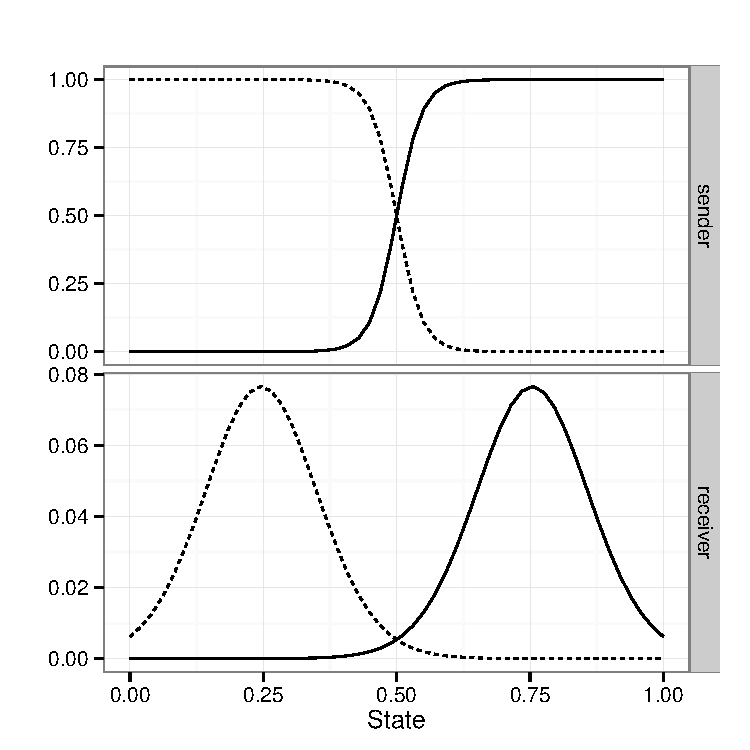
\includegraphics[width=\textwidth]{plots/exampleStratQRE_tolerance05.pdf}
    \caption{$\ns = 90$, $\lambda = 15$, $\toler = 0.5$}
    \label{fig:exampleQRE_stratsA}
  \end{subfigure}
  \hfill
  \begin{subfigure}[]{0.45\textwidth}
    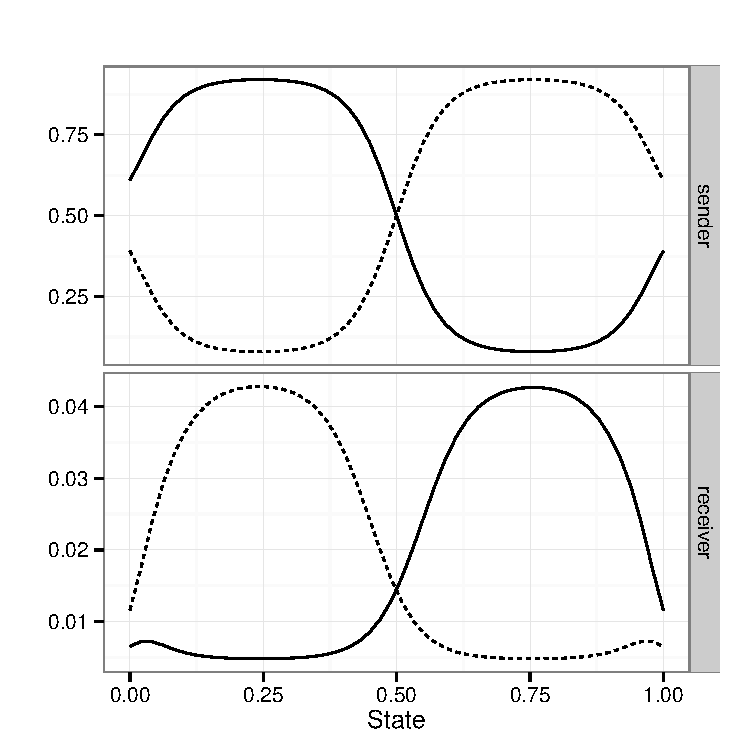
\includegraphics[width=\textwidth]{plots/exampleStratQRE_tolerance005.pdf}
    \caption{$\ns = 90$, $\lambda = 15$, $\toler = 0.05$}
    \label{fig:exampleQRE_stratsB}
  \end{subfigure}

  \caption{Examples of vague quantal response equilibria.}
  \label{fig:exampleQREs}
\end{figure}


But not all quantal response equilibria are equally plausible
explanations of vague language use, and the ones that are not suggest
that it is less plausible to think of vagueness as arising because of
errors in the computation and maximization of expected utility, as the
quantal response approach assumes, than that it arises due to
confusion of similar states, as the \rdd proposes. To see what the
problem is, we can look at cases like given in
Figure~\ref{fig:exampleQRE_stratsB}, which is the quantal response
equilibrium for a game with lower tolerance $\toler = 0.05$. Unlike
what evolves under \rdd in this case, sender strategies have vague
boundaries also towards the end of the unit intervals. Technically,
this is because quantal responses equalize message use far away from
the ``prototypical'' interpretation, not just in-between categories,
so to speak. This, in turn, is because quantal responses introduce
noise into the decision making at the level of computing or maximizing
expected utility of choices.

That this is conceptually odd shows even more clearly in a case where
the state space is intuitively unbounded, as for instance for the
property ``tall''. If the usual interpretation of a ``tall man'' peaks
at around, say, 195cm then when meeting a giant of $n$ meters speakers
would, according to the quantal response approach, be ever more
inclined to describe the giant indifferently as either ``tall'' or
``short'' the larger $n$ gets. This is because, as the distance from
the prototype increases for larger $n$, the difference between the
expected utilities of saying ``short'' or ``tall'' will converge to
zero. Whence that the quantal response approach would predict that
speakers would grow indifferent between choice of antonyms as $n$
grows, which seems weird. 

Admittedly, this argument hinges on the choice of utility
function. Still, to the extent that the chosen lower bounded utility
functions are reasonable ---and we think they are very reasonable---,
the case suggests that quantal responses are not a good model,
intuitively speaking, for why linguistic categories are
vague. Vagueness is more plausibly an effect of perceptual confusion
of similar states, than of computational errors in maximizing expected
utility.

%%% Local Variables: 
%%% mode: latex
%%% TeX-master: "paper"
%%% TeX-PDF-mode: t
%%% End:





\section{Conclusions}
\label{sec:conclusions}

It is a special case in the sense that the \rdd incorporates a
particular kind of mutation that is based on the similarity of states
(as defined in the sim-max game). More concretely, we start from the
idea that similar states are more easily confused than less similar
states. To formalize this idea, we assume that there is a confusion
matrix $C$, where $C_{ij}$ is the probability that a state \mystate{i}
is realized as a possibly different state \mystate{j}. (There is a
slightly different sense of ``realization'' in the sender and the
receiver side, and we will enlarge on this below.) Based on this, we
show two things. For one, we show how the discrete-time formulation of
the replicator dynamic can be easily adapted to integrate diffusion of
behavior due to confusion of states. This yields the \rdd in its basic
discrete-time formulation. For another, we also show that there exists
a translation of the confusion matrix $C$ into a suitable mutation
matrix $M_C$ such that the effect of $C$ and $M_C$ are ``equivalent''
in a sense to be made precise. This supports the conclusion that the
\rdd can indeed be thought of as a special case of the \rmd.

Based on data from numerical simulations, we show that the inclusion
of mild levels of such stochastic noise in the replicator dynamics
does not disrupt the possibility of evolving communicative efficient
signaling strategies at all. On the contrary, there might even be a
higher-order benefit to the presence of perceptual imprecision, in
that it accelerates converges, but also unifies and regularizes
evolutionary outcomes in such a way that inefficient categorization is
avoided. These results complement similar results by
\citet{OConnor2013:The-Evolution-o}, obtained for a micro-dynamic
extension of reinforcement learning. The \rdd adds to this a more
general, abstract framework that is not tied to the specific
assumptions of turn-based reinforcement. 

%%% Local Variables: 
%%% mode: latex
%%% TeX-master: "paper"
%%% TeX-PDF-mode: t
%%% End:





\appendix

\section{Proofs}
\label{sec:proofs}

\begin{proof}[Proof of Theorem~\ref{thm:sender-eq}]
  Fix $\Smixed$ and $\Sstrat = G(\Smixed)$. Look first at the rhs of
  the consequent:
  \begin{align*}
    C(\Sstrat)(\messg_y \probbar \state_x) & =  \sum_{\state_l} C_{xl}
    \cdot \Sstrat(\messg_y \probbar \state_l) \\
    & =  \sum_{\state_l} C_{xl}
    \cdot  \sum_{\Spure(\state_l) = \messg_y} \Smixed(\Spure) \\
    & = \sum_{\state_l}
    \sum_{\Spure(\state_l) = \messg_y} \Smixed(\Spure) \cdot C_{xl}\,.
  \end{align*}
  Next consider the lhs of the consequent:
  \begin{align*}
    G(Q^C(\Smixed))(\messg_y \probbar \state_x) & =
    \sum_{\Spure_i(\state_x)=\messg_y} Q^C(\Smixed)(\Spure_i) \\
    & = \sum_{\Spure_i(\state_x)=\messg_y} \sum_{\Spure_j}
    \Smixed(\Spure_j) \cdot Q^C_{ji} \\
    & = \sum_{\Spure_i(\state_x)=\messg_y} \sum_{\Spure_j}
    \Smixed(\Spure_j) \cdot \prod_{\state_l} \sum_{\state_m \in
      \Spure_j^{-1}(\Spure_i(\state_l))} C_{lm} \\
    & = \sum_{\Spure_j} \Smixed(\Spure_j) \cdot
    \sum_{\Spure_i(\state_x)=\messg_y} \prod_{\state_l}
    \sum_{\state_m \in \Spure_j^{-1}(\Spure_i(\state_l))} C_{lm}
  \end{align*}
  To simplify this further we look at a fixed $\Spure_j$ and consider
  the term: 
  \begin{align}
    \label{eq:term}
    \sum_{\Spure_i(\state_x)=\messg_y} \prod_{\state_l} \sum_{\state_m
      \in \Spure_j^{-1}(\Spure_i(\state_l))} C_{lm}\,.
  \end{align}
  Let $Y$ be the row-stochastic matrix with $Y_{kl} = \sum_{\state_m
    \in \Spure_j^{-1}(\messg_l)} C_{km}$. Every pure sender strategy
  maps each state $\state_k$ onto exactly one $Y_{kl}$. If we quantify
  over all pure strategies, we essentially look at each such
  mapping. Term (\ref{eq:term}) above quantifies over all pure
  strategies that map $\state_k$ onto $\messg_y$. The above term then
  sums over all products whose factors are tuples in $\times_{k>2}
  \set{y \setbar \exists l \mycolon y = Y_{kl}}$. So term
  (\ref{eq:term}) expands to (where $e = \card{\States}$ and $d=\card{\Messgs}$):
  \begin{align*}
    & (Y_{11} \cdot Y_{21} \cdot Y_{31} \cdot \ldots \cdot Y_{e1}) +
    (Y_{11} \cdot Y_{21} \cdot Y_{31} \cdot \ldots \cdot Y_{e2}) + 
    \dots \\
    & + (Y_{11} \cdot Y_{2d} \cdot
    Y_{3d} \cdot \ldots \cdot
    Y_{ed})\\
    = &    
  \end{align*}
  But since $Y$ is a row-stochastic matrix, this simplifies to
  $Y_{xy}$. Continuing the derivation with this:
  \begin{align*}
    G(Q^C(\Smixed))(\messg_y \probbar \state_x) 
    & = \sum_{\Spure_j} \Smixed(\Spure_j) \cdot
    \sum_{\state_l \in \Spure_j^{-1}(\messg_y)} C_{xl} \\
    & = \sum_{\Spure_j} \sum_{\state_l \in \Spure_j^{-1}(\messg_y)} \Smixed(\Spure_j) \cdot
     C_{xl} \\
     & = \sum_{\state_l}
    \sum_{\Spure(\state_l) = \messg_y} \Smixed(\Spure) \cdot C_{xl}\,.
  \end{align*}

\end{proof}

\begin{proof}[Proof of \ref{thm:receiver-eq} ]
  Fix $\Rmixed$ and $\Rstrat = G(\Rmixed)$. The rhs of the consequent
  expands to:
  \begin{align*}
    C(\Rstrat)(\state_x \probbar \messg_y) & = \sum_{\state_j}
    \sum_{i \in \set{k \setbar \Rpure_k(\messg_y) = \state_x}}
    \Rmixed_i \cdot C_{jx} \\
    & = \sum_{\Rpure_i} \sum_{j \in \set{k \setbar \Rpure_i(\messg_y) = \state_j}}
    \Rmixed_i \cdot C_{jx} \\
    & = \sum_{\Rpure_i} \Rmixed_i \cdot C_{\Rpure_i(\messg_y)x} \,.
  \end{align*}
  The rhs expands to:
  \begin{align*}
    G(R^C(\Rmixed))(\state_x \probbar \messg_y) & = \sum_{\Rpure_i}
    \Rmixed_i \cdot \sum_{j \in \set{j \setbar \Rpure_k(\messg_y) =
        \state_x}} 
    \prod_{\messg} C_{\Rpure_i(\messg)\Rpure_j(\messg)}
  \end{align*}
  Without loss of generality, assume that $x=y=1$, and fix
  $\card{M}=d$ and let $e$ be the number of pure receiver
  strategies. Then the last term can be rewritten as:
  \begin{align*}
    & = \sum_{i}
    \Rmixed_i \cdot ( C_{\Rpure_i(\messg_1)1} \cdot
      C_{\Rpure_i(\messg_2)\Rpure_1(\messg_2)} \cdot \ldots \cdot
      C_{\Rpure_i(\messg_d)\Rpure_1(\messg_d)} + \ldots  \\
      & \textcolor{white}{ = \sum_{i}
    \Rmixed_i  (}  +  C_{\Rpure_i(\messg_1)1} \cdot
      C_{\Rpure_i(\messg_2)\Rpure_2(\messg_2)} \cdot \ldots \cdot
      C_{\Rpure_i(\messg_d)\Rpure_2(\messg_d)} + \ldots  \\
      & \textcolor{white}{ = \sum_{i}
    \Rmixed_i  (}  + C_{\Rpure_i(\messg_1)1} \cdot
      C_{\Rpure_i(\messg_2)\Rpure_e(\messg_2)} \cdot \ldots \cdot
      C_{\Rpure_i(\messg_d)\Rpure_e(\messg_d)}) )
  \end{align*}
  Every for every messages $C_{\Rpure_i(\messg_l)}$ is a stochastic
  vector. For $l>1$, all elements of these vectors appear equally
  often. But that means that these cancel out. What remains is:
  \begin{align*}
    & = \sum_{\Rpure_i} \Rmixed_i \cdot C_{\Rpure_i(\messg_y)x} \,.
  \end{align*}
\end{proof}


%%% Local Variables: 
%%% mode: latex
%%% TeX-master: "paper"
%%% TeX-PDF-mode: t
%%% End:






\printbibliography[heading=bibintoc]

\end{document}
